\chapter{Use cases with Simplified tools}


%-------------------------------------------------------------------
%-------------------------------------------------------------------
%-------------------------------------------------------------------

\section{The Vincennes data set}

%-------------------------------------------------------------------

\subsection{Description of the data set}
\label{Vincennes:DataSet}

On {\tt micmac\_data/ExempleDoc/} the directory {\tt Vincennes} contains
$106$ images of the Vincennes's castel \footnote{they are low resolution images
to limit the  downloading time}. This data set illustrate how
the tools described here can be used to achieve a typical architectural task:
compute for each of the main facade an ortho photo, these ortho photo
must be referenced in the same coordinate system.  Although the ortho-cylindric
option for geometry described to process thi acquisition seems a very specific
and narrow technical case, practically it corresponds to very current case
for facade processing.


The $106$ images of Vincenne's data set are organized in $4$ subset :


\begin{itemize}
   \item  images {\tt Face1.*} correspond to the first facade;
   \item  images {\tt Face2.*} correspond to the second facade;
   \item  images {\tt  Lnk12.*} images acquired to make the link between
           the two facades;
   \item  images {\tt  Calib.*} acquired to have easily a first
           calibration.
\end{itemize}

Note that, \emph{before any processing}, the images have been renamed taking 
into account the acquisition structure. It is highly recommanded to do the
same thing before processing data sets having some complexity. It avoids
the creation of tricky regular expression. These images are jpeg low resolution
images to limit the bandwith when one upload the data, but of course in
real case the full resolution raw image will be prefered.


\begin{figure}
\begin{center}
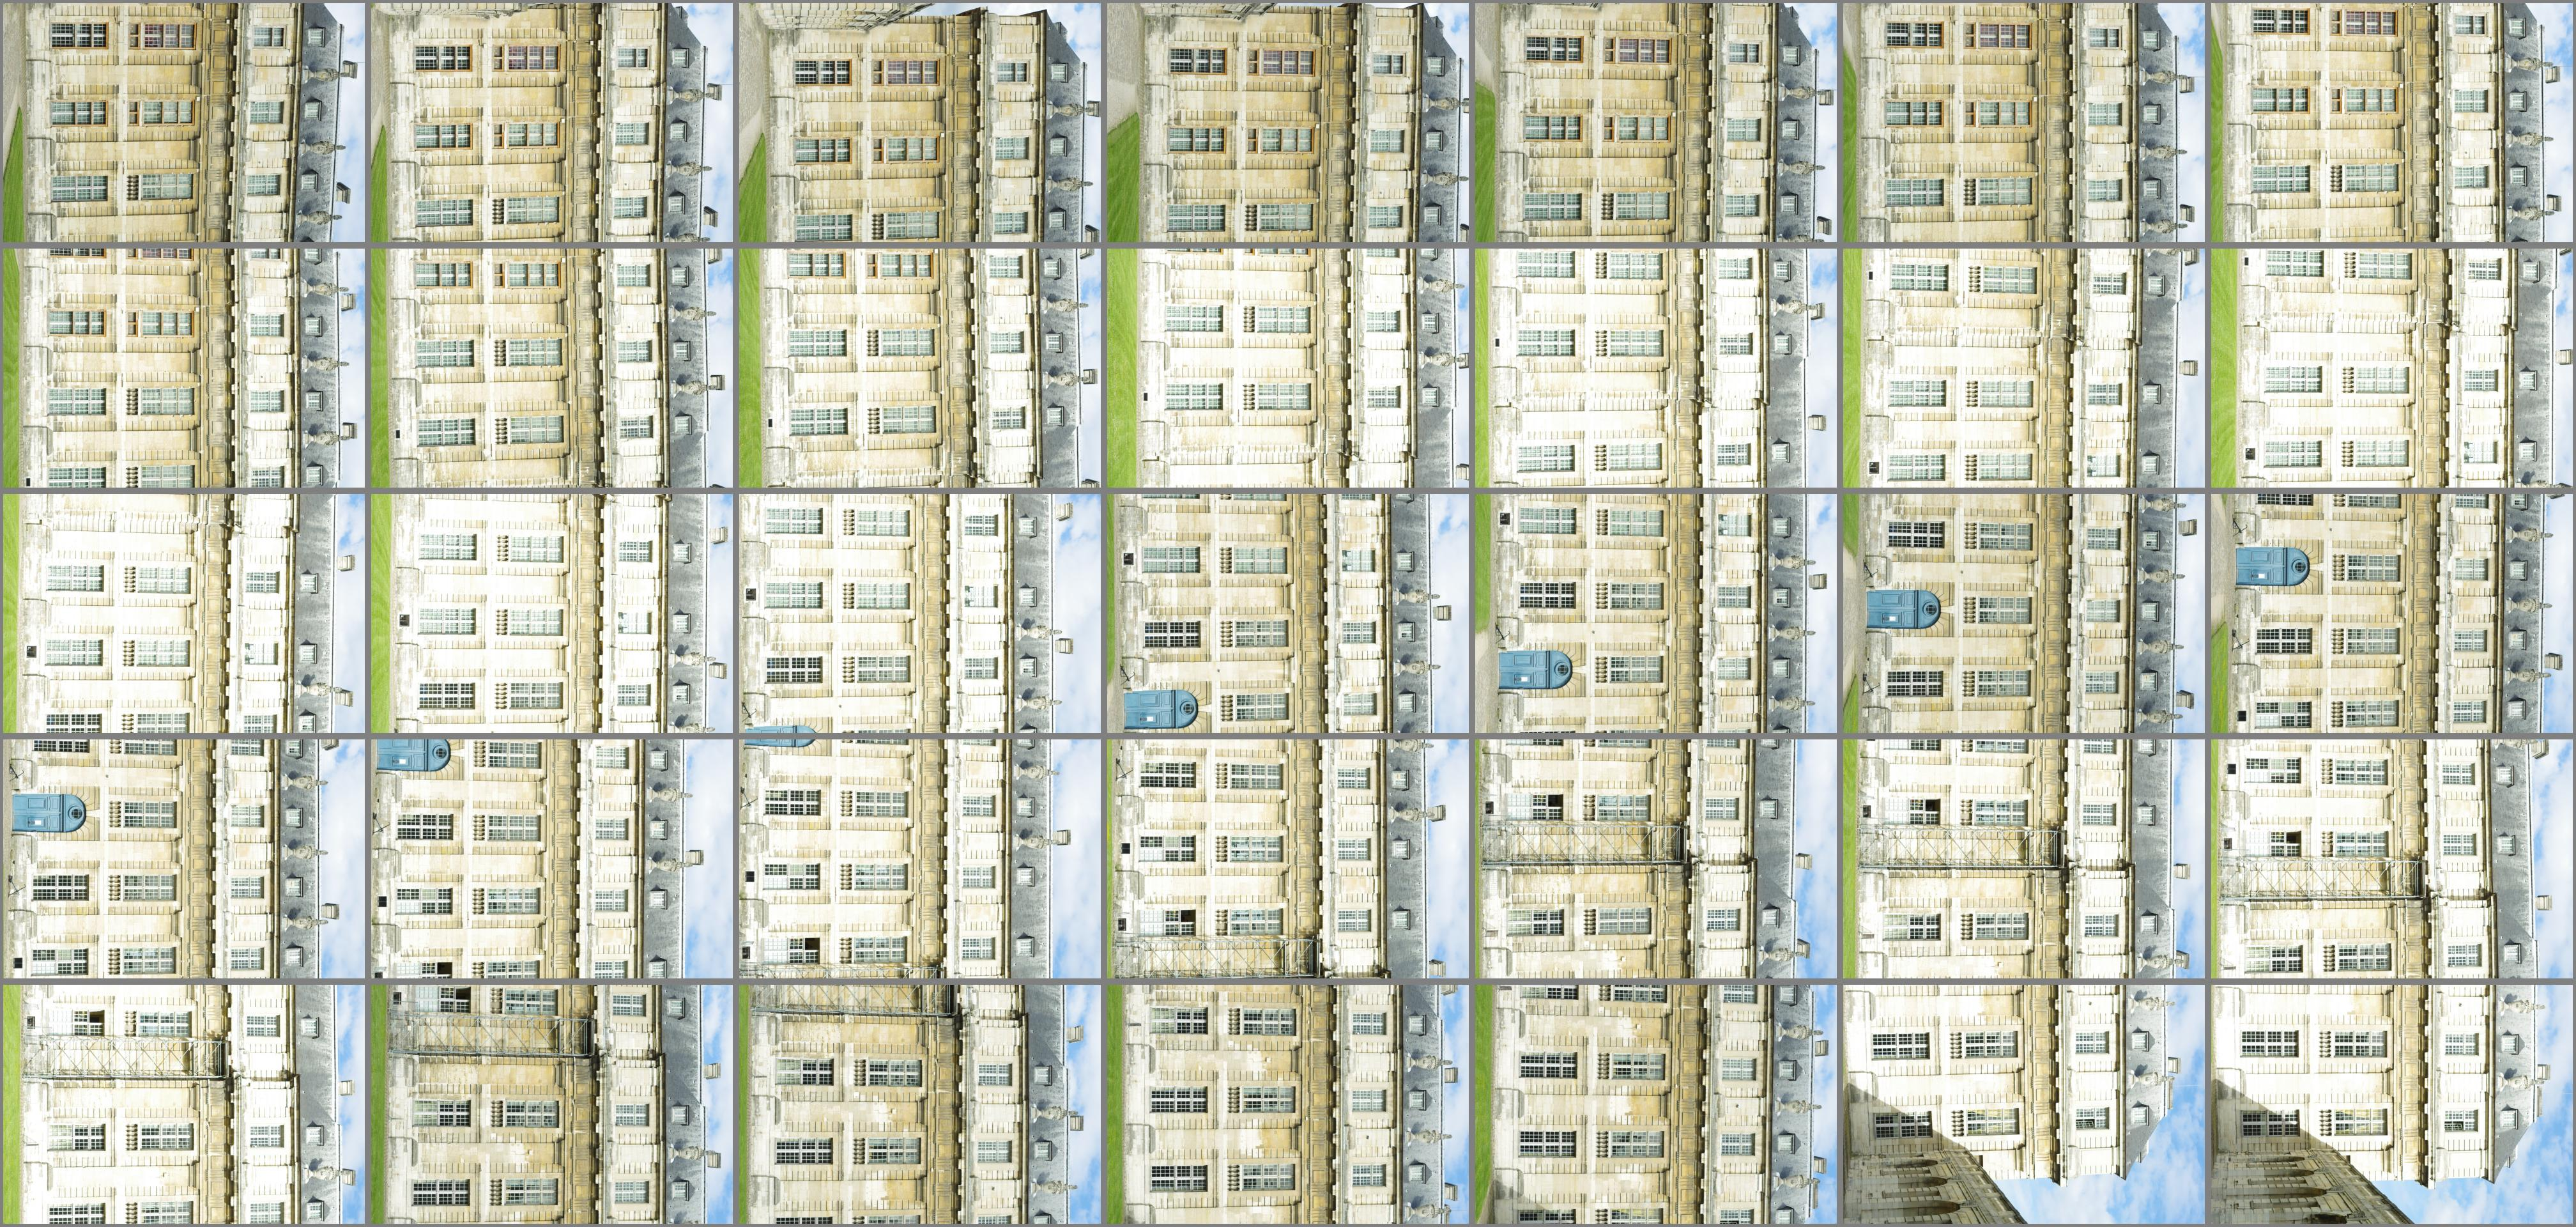
\includegraphics[width=120mm]{FIGS/Vincennes/Planche-F1.jpg}

\vspace{0.3cm}
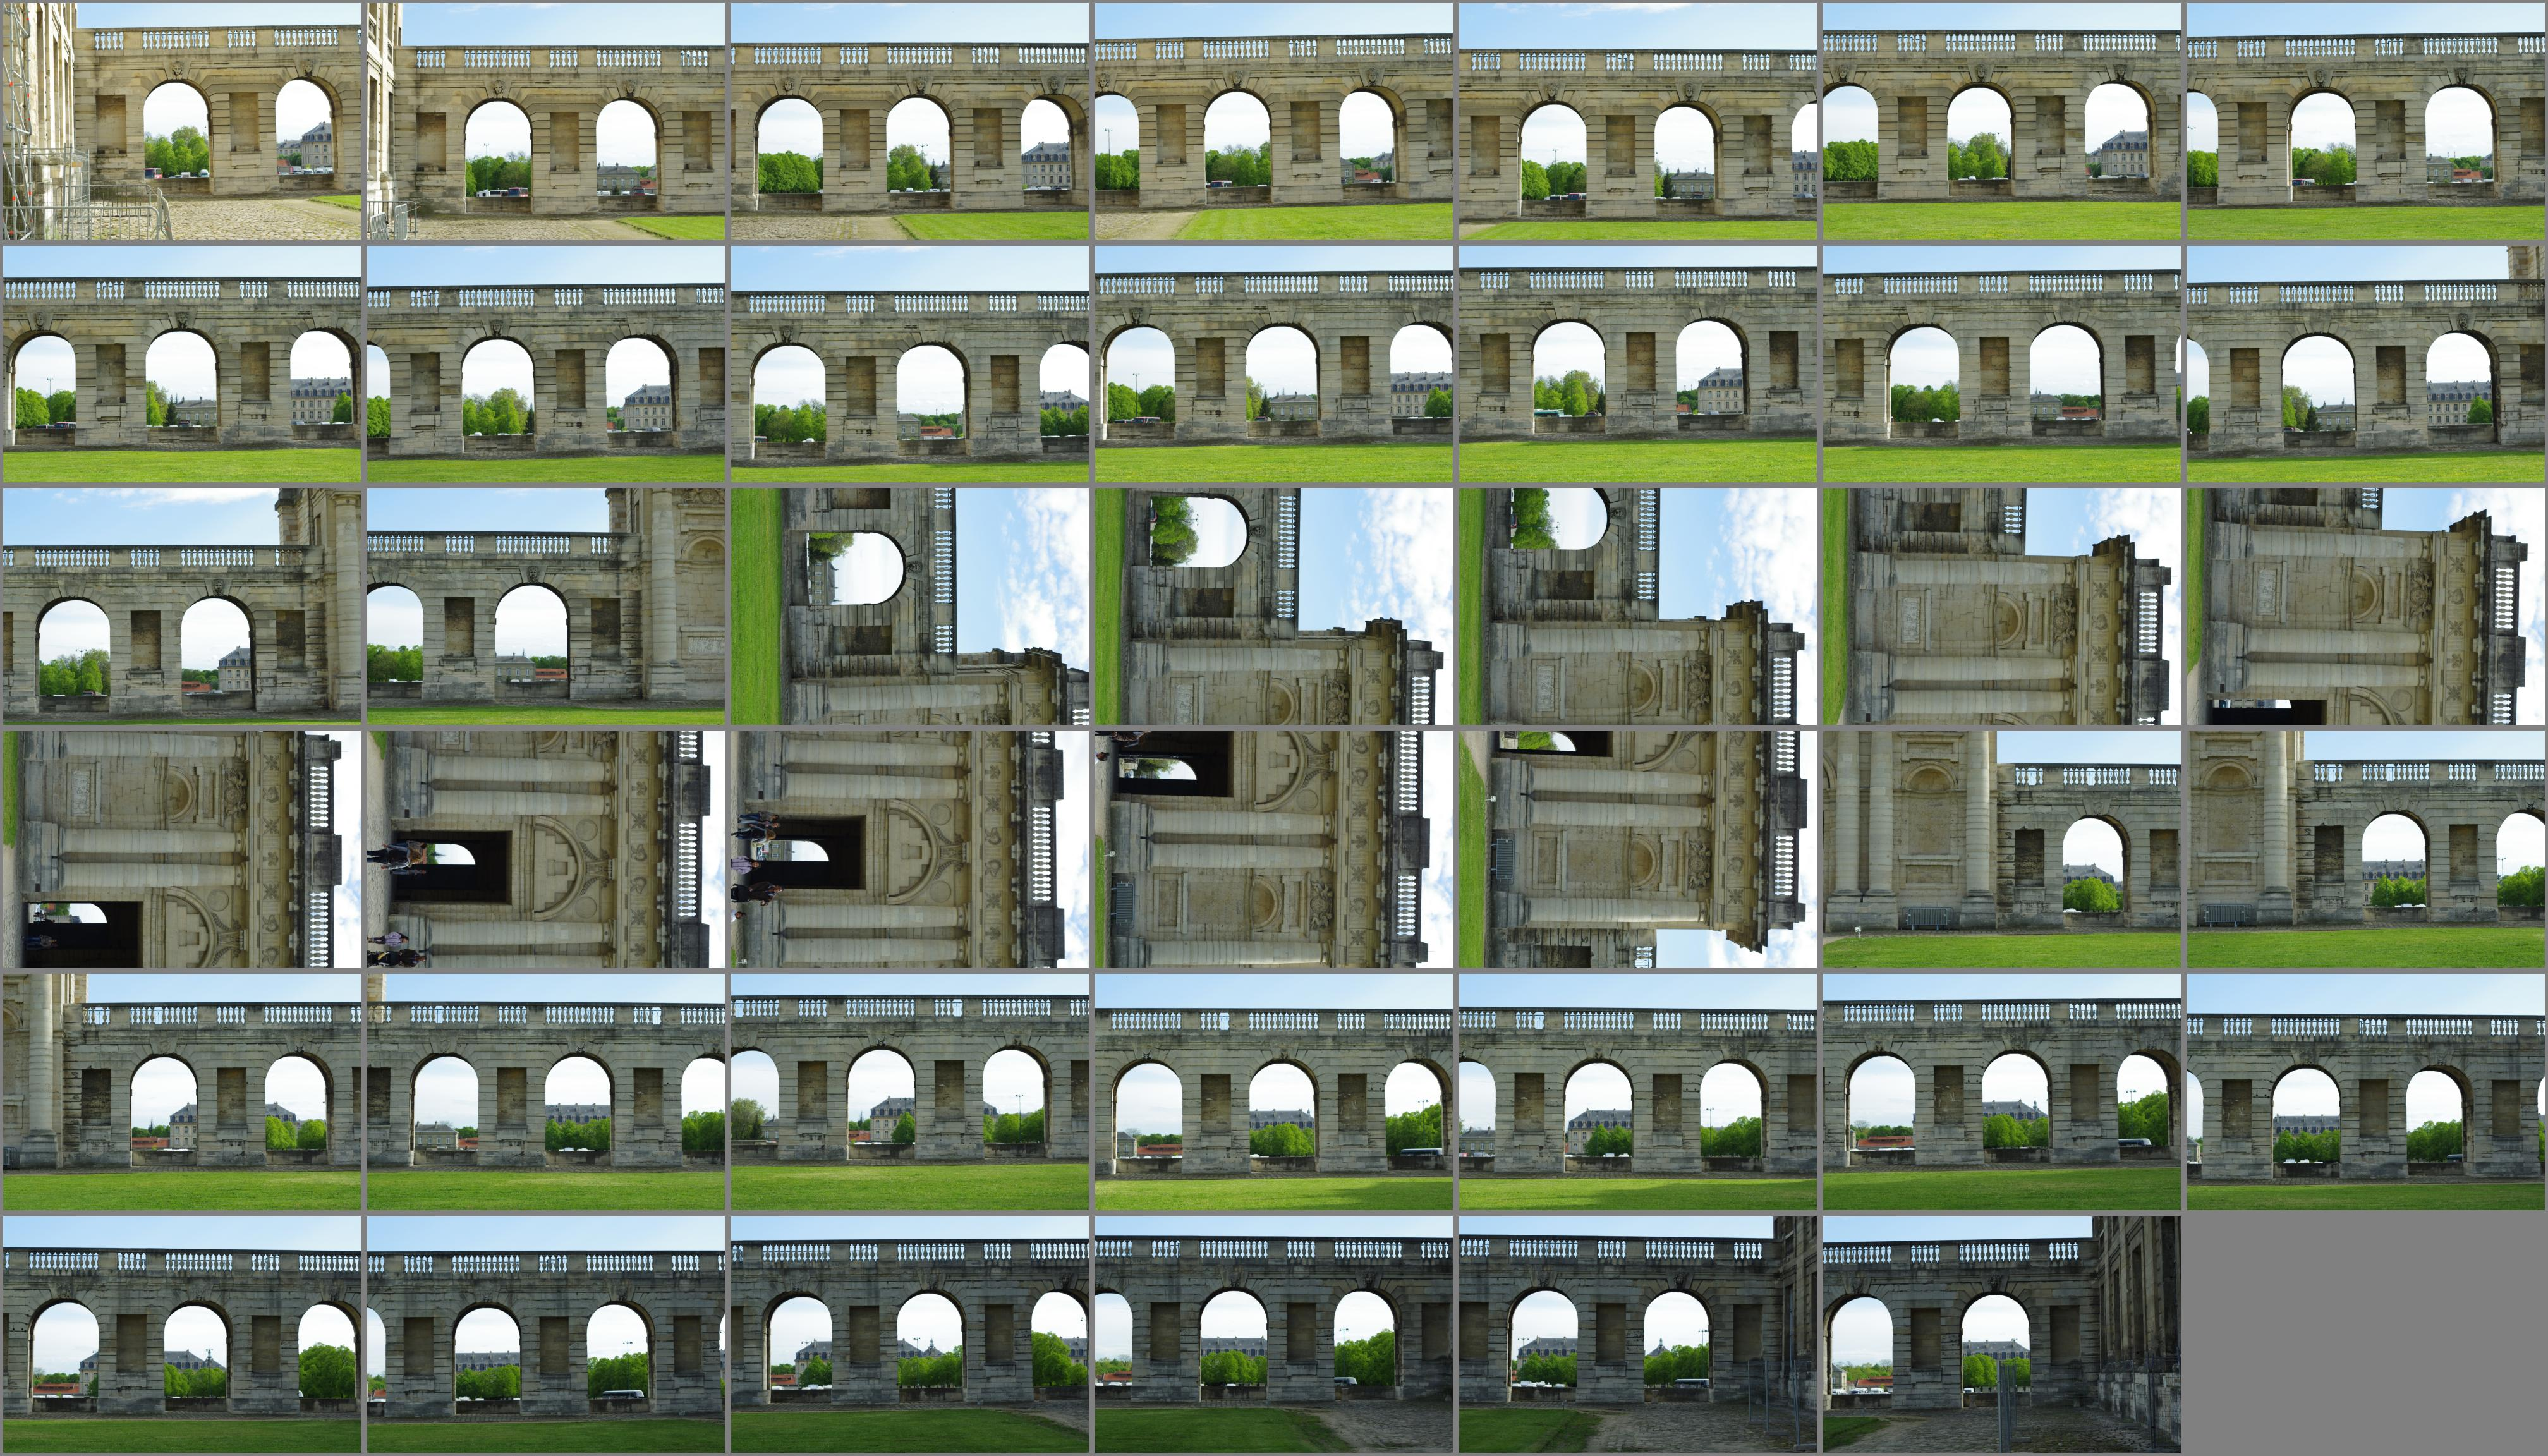
\includegraphics[width=120mm]{FIGS/Vincennes/Planche-F2.jpg}

\vspace{0.3cm}
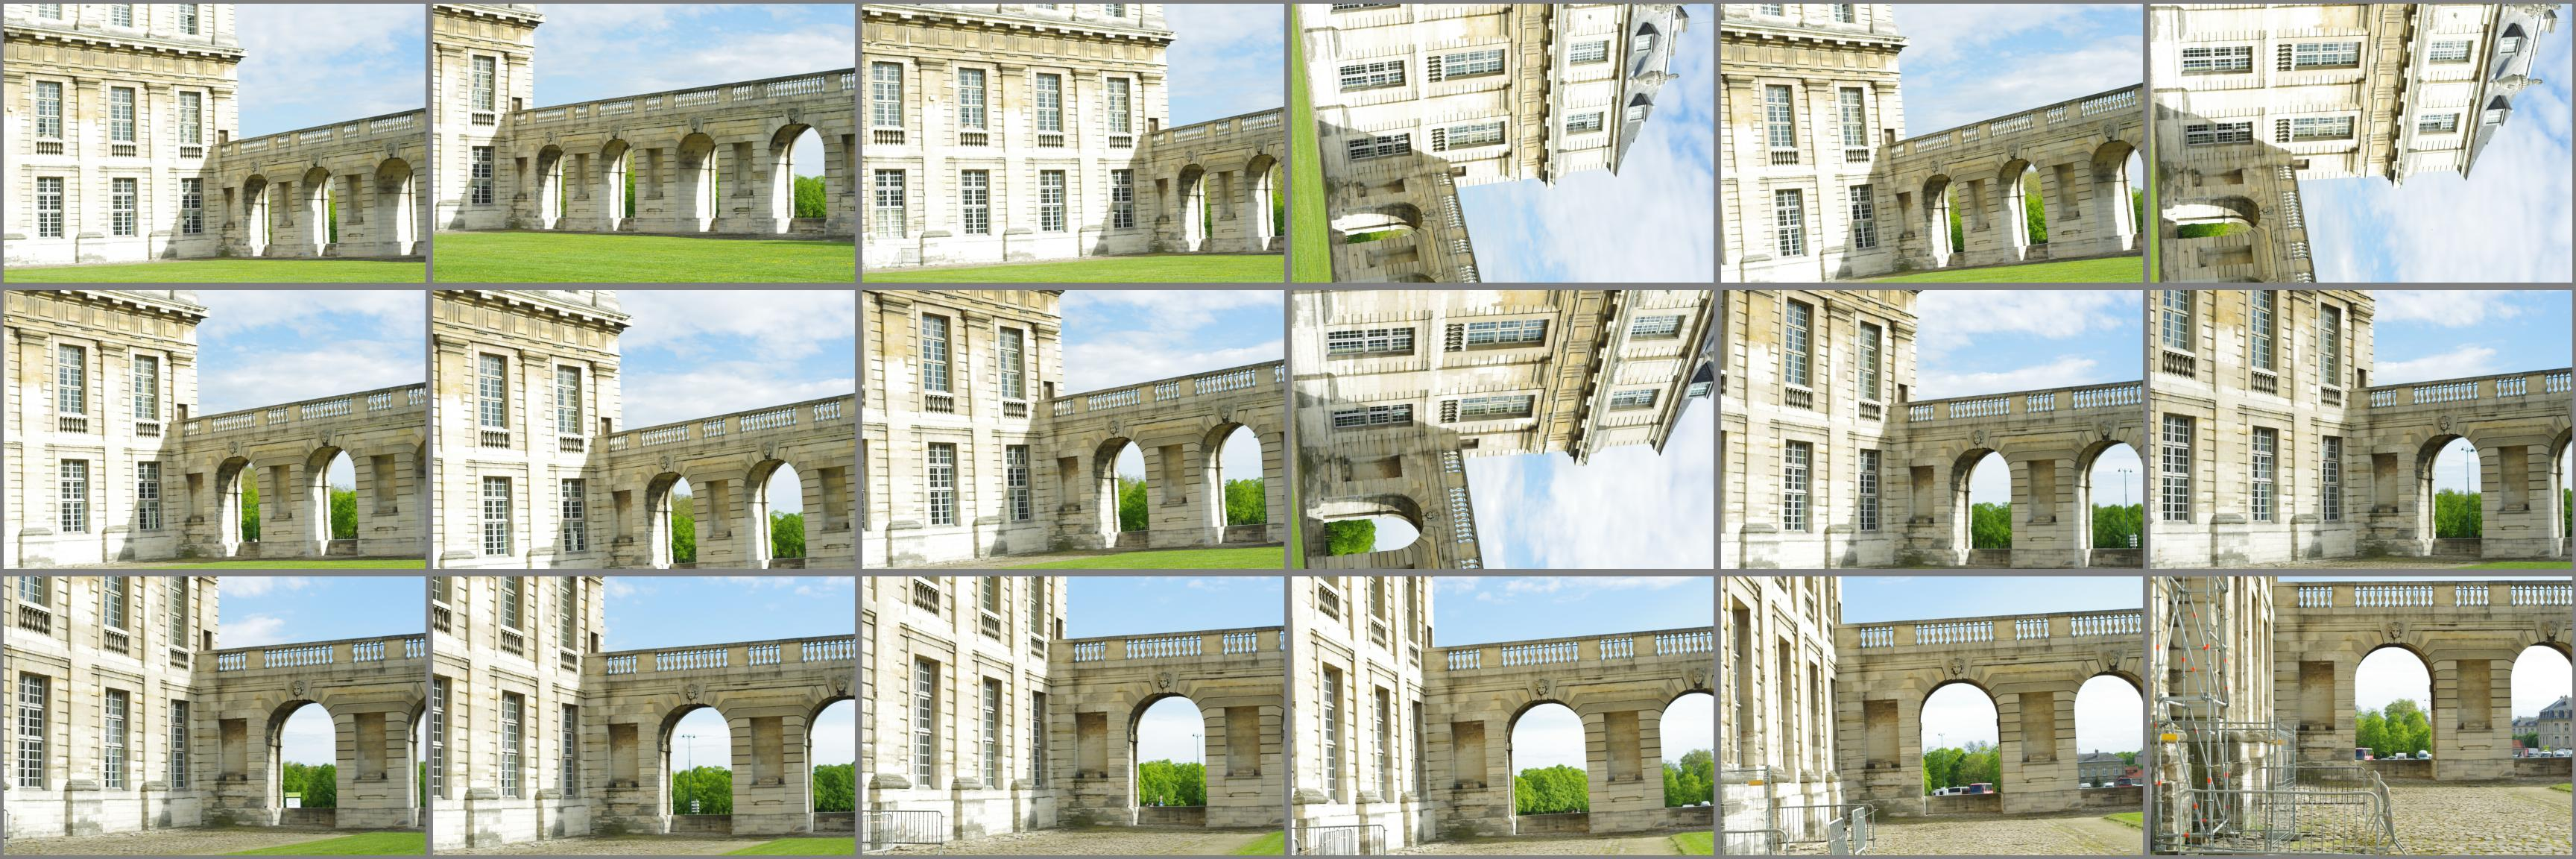
\includegraphics[width=120mm]{FIGS/Vincennes/Planche-Lnk.jpg}

\vspace{0.3cm}
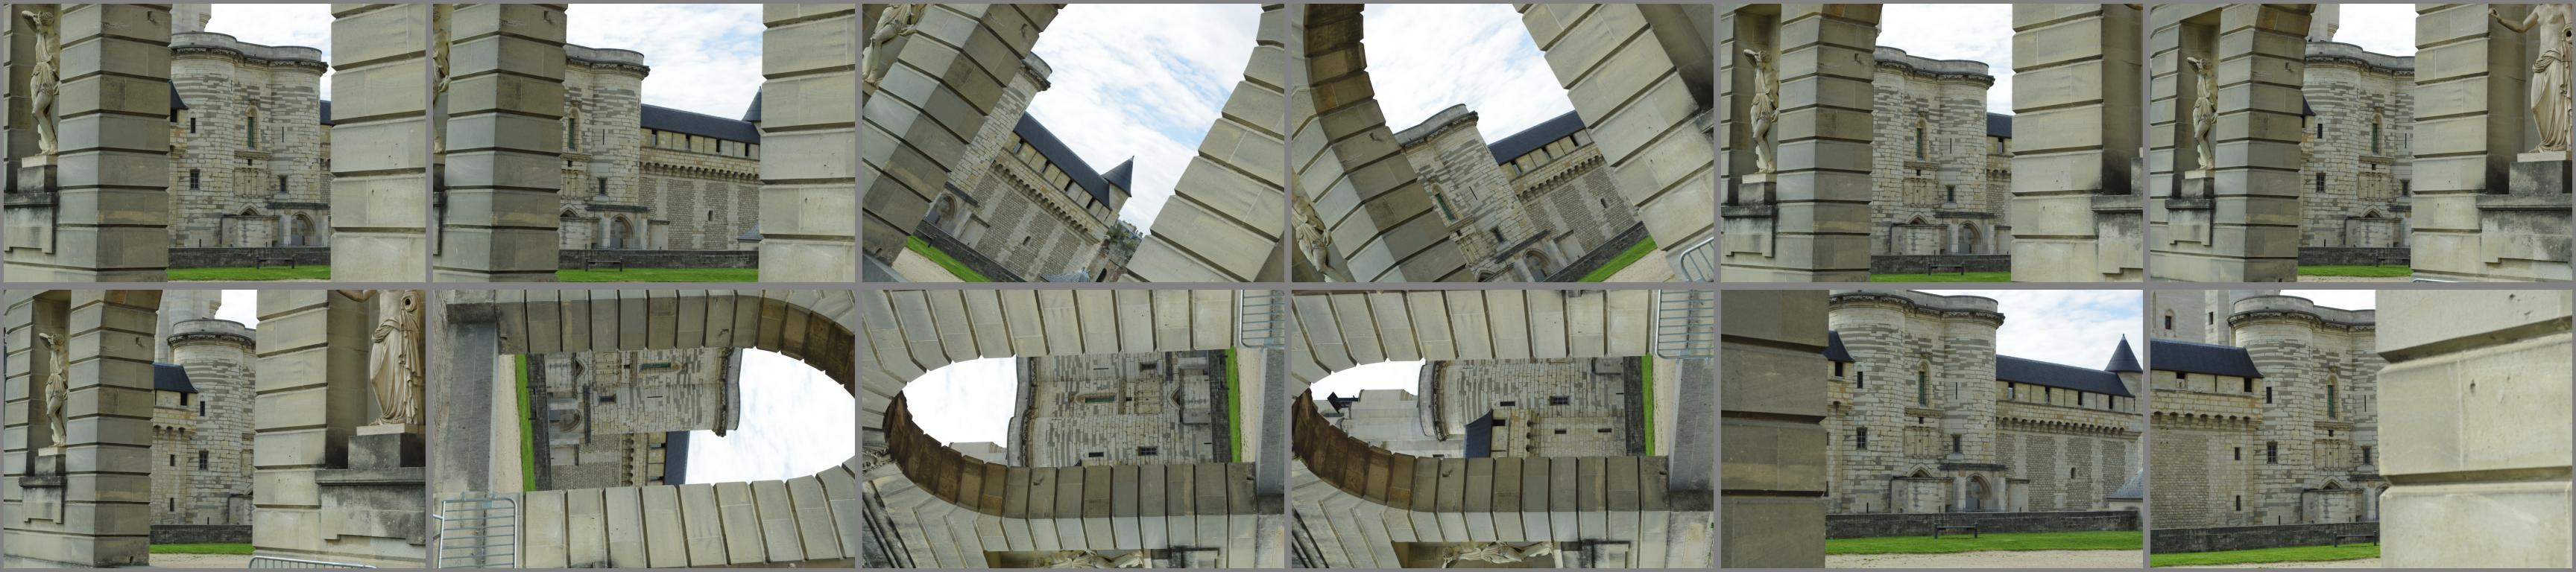
\includegraphics[width=120mm]{FIGS/Vincennes/Planche-Calib.jpg}
\end{center}
\caption{Image of Vincenne's data set : Face1, Face2, Lnk12 and Calib }
\label{FIG:Glob:Vincenne}
\end{figure}




The file {\tt  ExeCmd.txt} contains all the commands that we will need to process these images.


%-------------------------------------------------------------------

\subsection{Computing tie points and orientations}

    %  -  -  -  -  -  -  -  -  -  -  -  -

\subsubsection{Tie points}

The computation of tie points and relative orientation is quite
classic now. 

For tie points we want to compute:

\begin{itemize}
   \item  points  between all pairs of calibration data set;
   \item  points  of \emph{Face1} and \emph{Face2} using the linear structure of
          the aqcuisition;
   \item  points  between \emph{Lnk12} and connected subset of  \emph{Face1} and \emph{Face2};
\end{itemize}

This is done by :

\begin{verbatim}
Tapioca All  "Calib-IMGP[0-9]{4}.JPG" 1000
Tapioca Line "Face1-IMGP[0-9]{4}.JPG" 1000 5
Tapioca Line "Face2-IMGP[0-9]{4}.JPG" 1000 5
Tapioca All  "((Lnk12-IMGP[0-9]{4})|(Face1-IMGP529[0-9])|(Face2-IMGP531[0-9])).JPG" 1000
\end{verbatim}

    %  -  -  -  -  -  -  -  -  -  -  -  -

\subsubsection{Relative orientation}

Then we want to make a first calibration with the calibration data set, and
use this calibration as an initial value to the global orientation of
\emph{Face1},  \emph{Face2} and \emph{Lnk12}. This is done by :

\begin{verbatim}
Tapas RadialStd "Calib-IMGP[0-9]{4}.JPG" Out=Calib
Tapas RadialStd "(Face1|Face2|Lnk12)-IMGP[0-9]{4}.JPG" Out=All InCal=Calib
\end{verbatim}

    %  -  -  -  -  -  -  -  -  -  -  -  -

\subsubsection{Optional, absolute orientation}

Finally, we want to transform the orientation from an arbitrary relative 
orientation to some physically based orientation. If we have some ground
control points, this can be done using the {\tt GCPBascule} command (see~\ref{Sec:GCPBascule}) . To
generate orientation in {\tt Ori-Ground} :

\begin{verbatim}
GCPBascule  "(Face1|Face2|Lnk12)-IMGP[0-9]{4}.JPG" All Ground Mesure-TestApInit-3D.xml\
 Mesure-TestApInit.xml
\end{verbatim}

    %  -  -  -  -  -  -  -  -  -  -  -  -

\subsubsection{Optional, scene-based orientation}

Alternatively, if we do not have any GCP and want to put the data in an orientation
having some physical meaning, we can use the {\tt SBGlobBascule} command (see~\ref{ScBas:Basc}) :

\begin{verbatim}
SBGlobBascule "(Face1|Face2|Lnk12)-IMGP[0-9]{4}.JPG" All MesureBascFace1.xml  Glob \
    PostPlan=_MasqPlanFace1  DistFS=2.0 Rep=ij
\end{verbatim}

There is a new option {\tt Rep=ij}, the meaning of this option is :
\label{SGB:Rep}

\begin{itemize}
   \item it is a string that describe a repair;
   \item it must contain $2$ symbols, each symbols can be in \emph{\{i,-i,j,-j,k,-k\}} and desribe a vector;
   \item the globlal orientation with be such that in the final orientation the line 
         defined by {\tt Line1-Line2} is aligned on first vector, and the normal to the plane is aligned on second vector;
   \item here in final orientation $i$ will be the horizontal of the wall and $j$ will be the
         normal to the wall, consequently $k=i\wedge j$ will be the vertical;
\end{itemize}


%-------------------------------------------------------------------
\subsection{Matching}


    %  -  -  -  -  -  -  -  -  -  -  -  -
\subsubsection{"Standard" option}

The "standard pipeline" for generating an ortho photo of facade, 
as seen in~\ref{Simp:Tool:One}, is for each facade :

\begin{itemize} 
   \item compute a local repair to define the facade with {\tt RepLocBascule};
   \item compute a rectified image with {\tt Tarama}; 
   \item make the matching with {\tt Malt};
   \item generate the ortho image with {\tt  Tawny};
\end{itemize} 

This can be done by the succession of commands:

\begin{verbatim}
RepLocBascule  "(Face1)-IMGP[0-9]{4}.JPG" Ground  MesureBascFace1.xml Repere-F1.xml\
       PostPlan=_MasqPlanFace1
Tarama  "(Face1)-IMGP[0-9]{4}.JPG" Ground  Repere=Repere-F1.xml  Out=TA-F1 Zoom=4
Malt Ortho  "(Face1)-IMGP[0-9]{4}.JPG"  Ground  Repere=Repere-F1.xml  \
                     SzW=1 ZoomF=1  DirMEC=Malt-F1 DirTA=TA-F1
Tawny Ortho-Malt-F1/
\end{verbatim}

The results are quite deceiving !!! Figure~\ref{FIG:Pb:Vincenne} illustrate the
encountered problem :

\begin{itemize}
    \item on firt line, the ortho photo; it suffer several problem; the main problem
         are located on the roof (due to bad incidence angles) and on horizontal lines;

    \item on second line, a snapshot from Meshlab, showing the camera position;
          it illustrates the fact that in this acquisition all the camera centers are 
         located on the same line;

    \item the third line, focus on the matching problem  that occurs on linear detail that
          are parallel to the line of acquisition; 
\end{itemize}


\begin{figure}
\begin{center}
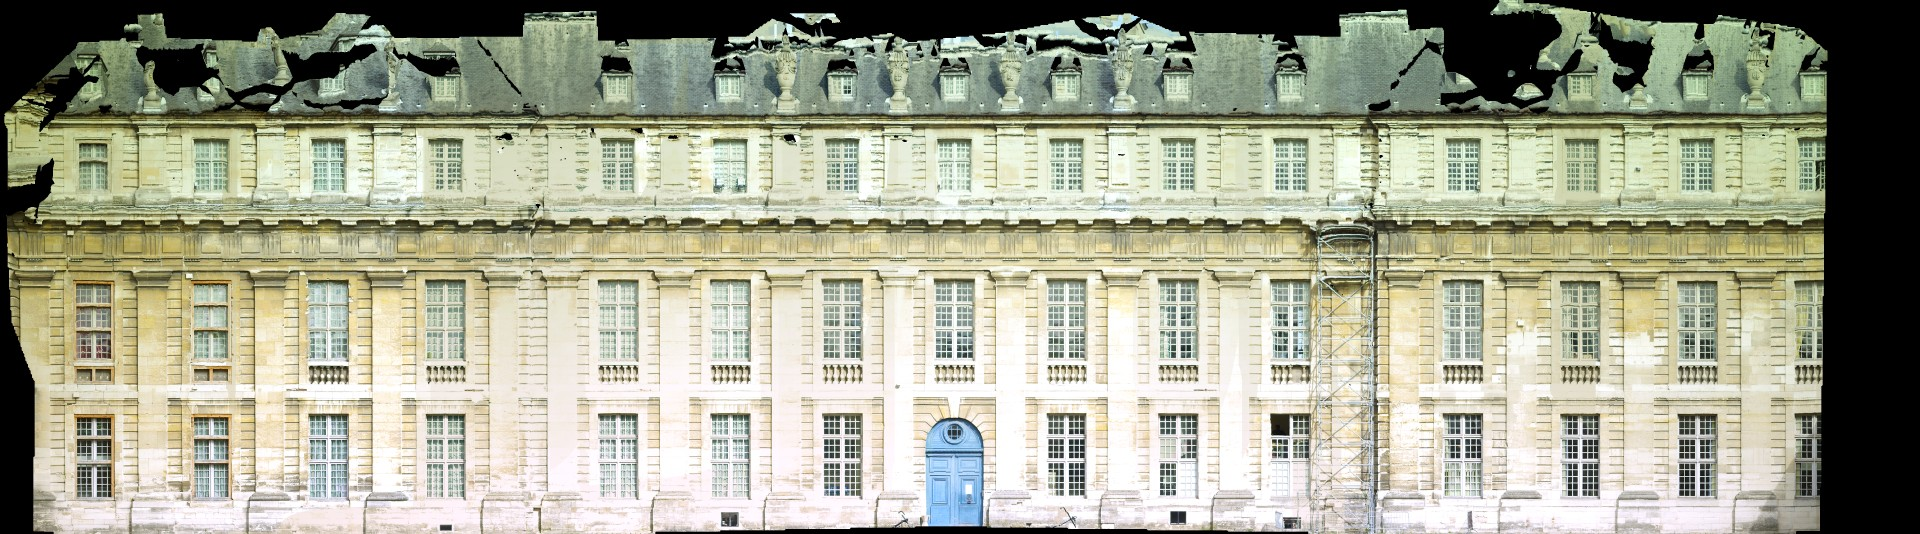
\includegraphics[width=160mm]{FIGS/Vincennes/Ortho-Moche.jpg}

\vspace{0.3cm}
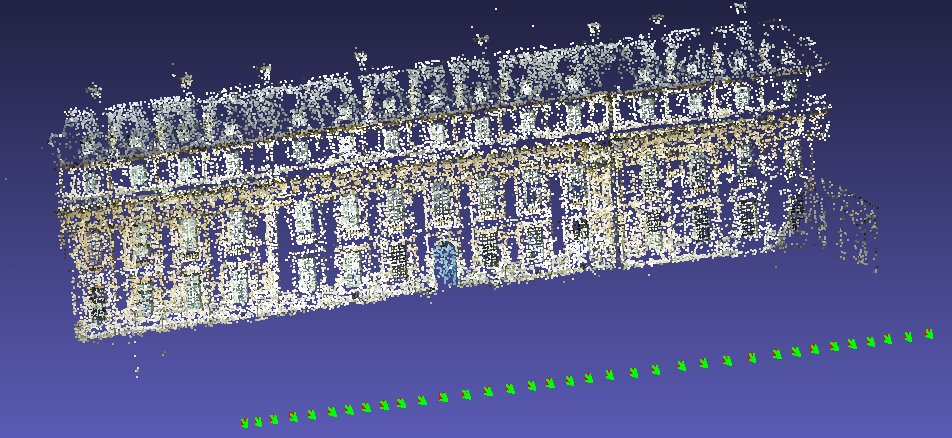
\includegraphics[width=160mm]{FIGS/Vincennes/CamFace1.jpg}

\vspace{0.3cm}
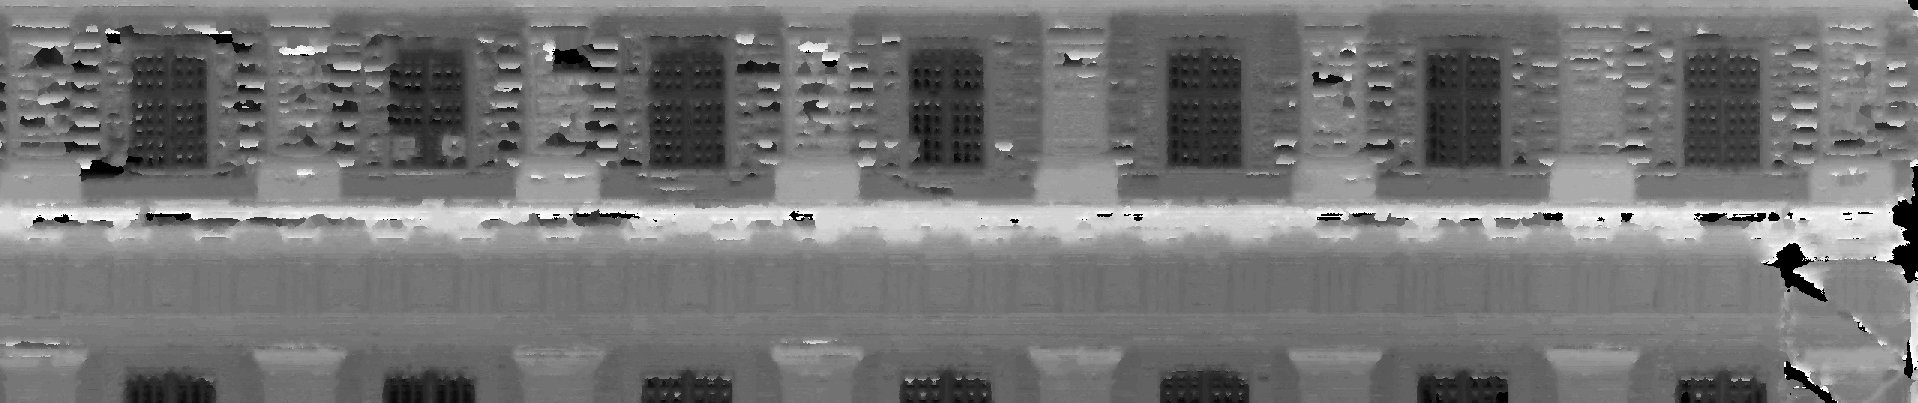
\includegraphics[width=160mm]{FIGS/Vincennes/MNT-Moche.jpg}

\end{center}
\caption{Problem with standard processing on Vincennes Facade : low quality ortho photo,
aligment of cameras, poor dept map especially for linear structure parallel to camera alignment}
\label{FIG:Pb:Vincenne}
\end{figure}


    %  -  -  -  -  -  -  -  -  -  -  -  -
\subsubsection{"Ortho-cylindric" option}

Intutively it  is obvious that when the camera center are all aligned on the same line,
the matching problem is  ambiguous for line parallel to the acquisition, consequently
the quality of result is poor. 
Obviously, the default would decrease (in fact disappear) if the camera were not
aligned, using an UAV or a scaffolding , we could have an optimal geometry similar
to aerial acquisition. But it is not always possible to have such material and, for economical reason, 
it would be interesting to be abble to obtain a relatively good quality ortho photo even when
all the camera are aligned.

In fact for theoretical reasons described in~\cite{Penard},
this problem are  much more important in ground geometry than in image geometry.
With the option we have seen until now, we have basically this alternative:

\begin{itemize}
   \item  use the ground geometry with a simple process but obtain bad qualitiy results such those of 
          figure~\ref{FIG:Pb:Vincenne};

   \item  use the image geometry with  good results but have a complicated workflow with many depth map
          that must be merged.
\end{itemize}


With such acquisition, the ortho-cylindrical geometry combine the benefit of these
two geometries. Intuitively this geometry is equivalent to the geometry of a virtual push-broom
camera, the line of this virtual push-broom being the line on which are located the 
camera center. More formally :


\begin{itemize}
   \item  let  $X,Y,Z$ be a coordinate system such that $Y=0$ be approximatively the line on which the camera
          are located, and $Z=D$ be approximatively the plane of the wall;

   \item  let  $U,V,L$ be the coordinate system defined by
\begin{itemize}
    \item  $U= D \tan^{-1} (\frac{X}{Z})$
    \item  $V=Y$ and $L=Z$;
\end{itemize}
   \item   we  will then compute the DSM as a function $L= F(U,V)$.
\end{itemize}

To use this geometry, we just need to set {\tt OrthoCyl=true} in the command {\tt RepLocBascule} :

\begin{verbatim}
RepLocBascule  "(Face1)-IMGP[0-9]{4}.JPG" Ground  MesureBascFace1.xml Ortho-Cyl1.xml\
   PostPlan=_MasqPlanFace1 OrthoCyl=true
\end{verbatim}

With this option, {\tt RepLocBascule} will also compute, using least mean square,
the line that fit the best the alignment of camera perspective centers. If we take 
a look at file {\tt Ortho-Cyl1.xml} we can see  this line coded by {\tt <P0>}
and {\tt <P1>}  (plus the previous local repair  {\tt <Repere>}) :

\begin{verbatim}
<XmlModeleSurfaceComplexe>
     <XmlOneSurfaceAnalytique>
          <XmlDescriptionAnalytique>
               <OrthoCyl>
                    <Repere>
                         <Ori>-0.00573  -2.7113574  -0.4521156 </Ori>
                         <Ox>  0.00029   0.9999998  -0.0003715 </Ox>
                         <Oy> -0.00043   0.0003716   0.9999998 </Oy>
                         <Oz>  0.99999  -0.0002960   0.0004372 </Oz>
                    </Repere>
                    <P0>30.392821 -2.720358 -0.438823</P0>
                    <P1>30.391561 -1.720359 -0.43974</P1>
                    <AngulCorr>true</AngulCorr>
               </OrthoCyl>
          </XmlDescriptionAnalytique>
          <Id>TheSurf</Id>
          <VueDeLExterieur>true</VueDeLExterieur>
     </XmlOneSurfaceAnalytique>
</XmlModeleSurfaceComplexe>
\end{verbatim}

    %  -  -  -  -  -  -  -  -  -  -  -  -
\subsubsection{Concrete use of "Ortho-cylindric" option}

It is then sufficient to give the file created by  {\tt RepLocBascule} 
as an optional parameter to {\tt Tarama} and {\tt Malt} to compute 
in the adequate geometry; for facade one, we can enter:


\begin{verbatim}
RepLocBascule  "(Face1)-IMGP[0-9]{4}.JPG" Ground  MesureBascFace1.xml Ortho-Cyl1.xml \
        PostPlan=_MasqPlanFace1 OrthoCyl=true
Tarama  "(Face1)-IMGP[0-9]{4}.JPG" Ground  Repere=Ortho-Cyl1.xml  Out=TA-OC-F1 Zoom=4
Malt Ortho  "(Face1)-IMGP[0-9]{4}.JPG"  Ground  Repere=Ortho-Cyl1.xml  \
                   SzW=1 ZoomF=1  DirMEC=Malt-OC-F1 DirTA=TA-OC-F1
Tawny Ortho-UnAnam-Malt-OC-F1/
\end{verbatim}

And for facade 2 :

\begin{verbatim}
RepLocBascule  "(Face2)-IMGP[0-9]{4}.JPG" Ground  MesureBascFace2.xml Ortho-Cyl2.xml \
     PostPlan=_MasqPlanFace2 OrthoCyl=true
Tarama  "(Face2)-IMGP[0-9]{4}.JPG" Ground  Repere=Ortho-Cyl2.xml  Out=TA-OC-F2 Zoom=4
Malt Ortho  "(Face2)-IMGP[0-9]{4}.JPG"  Ground  Repere=Ortho-Cyl2.xml  SzW=1 ZoomF=1  \
          DirMEC=Malt-OC-F2 DirTA=TA-OC-F2 NbVI=2
Tawny Ortho-UnAnam-Malt-OC-F2/
\end{verbatim}

Note some options of these commands:

\begin{itemize}
   \item in {\tt RepLocBascule}, the {\tt OrthoCyl=true} as described above;
   \item in {\tt Tarama}, the {\tt Out=TA-OC-F1} (and {\tt Out=TA-OC-F2}) to specify the
         directory of output; this is naturally to avoid that each call to {\tt Tarama} overwrite
         the result of previous calls;
   \item in {\tt Malt}, the {\tt DirTA=TA-OC-F1} to get the adequete entry from  {\tt Tarama} 
         and {\tt Out=DirMEC=Malt-OC-F1} to specify the results; this change the place are written
         the results of matching, and also the result of individual ortho photo (here it will be 
         {\tt Ortho-UnAnam-Malt-OC-F1/});
\end{itemize}


If the ortho-cylindric geometry is "optimal" for computation, this is 
generally not a proper geometry for the final user , so at the end of the process,
{\tt MicMac} generate an "un-anamorphosed" version of this depth map in
euclidean geometry.  For example on directory {\tt Malt-OC-F1/}, there
exists $9$ files {\tt Z\_NumX\_DeZoomY\_STD-MALT.tif} corresponding to
the different level of matching in ortho-cylindrical geometry, 
and a single file {\tt Z\_Num1\_DeZoom1\_Malt-Ortho-UnAnam.tif}
corresponding to the eulidean version of the last file
( this is the version presented on second line of
figure~\ref{FIG:OK:Vincenne}).
Note that in general there will be very few hidden part on 
ortho-cylindrical depth map; conversely, they are quite current on
euclidean version, but it is intrinsic to what we want to restituate
with such acquisition.
By default, the ortho photo are also generated in euclidean geometry
using the unanamorphosed depth-map. Here for example, they are
generated under {\tt Ortho-UnAnam-Malt-OC-F1/} and {\tt Ortho-UnAnam-Malt-OC-F2/}.


Figure~\ref{FIG:OK:Vincenne} present some results obtained after this process:

\begin{itemize}
    \item first line present the depth-map computed in ortho-cylindric geometry using
           color code;
    \item  second line, euclidean version of the depth map, remark the hidden part;

    \item  third line, ortho photo of facade.
\end{itemize}

\begin{figure}
\begin{center}
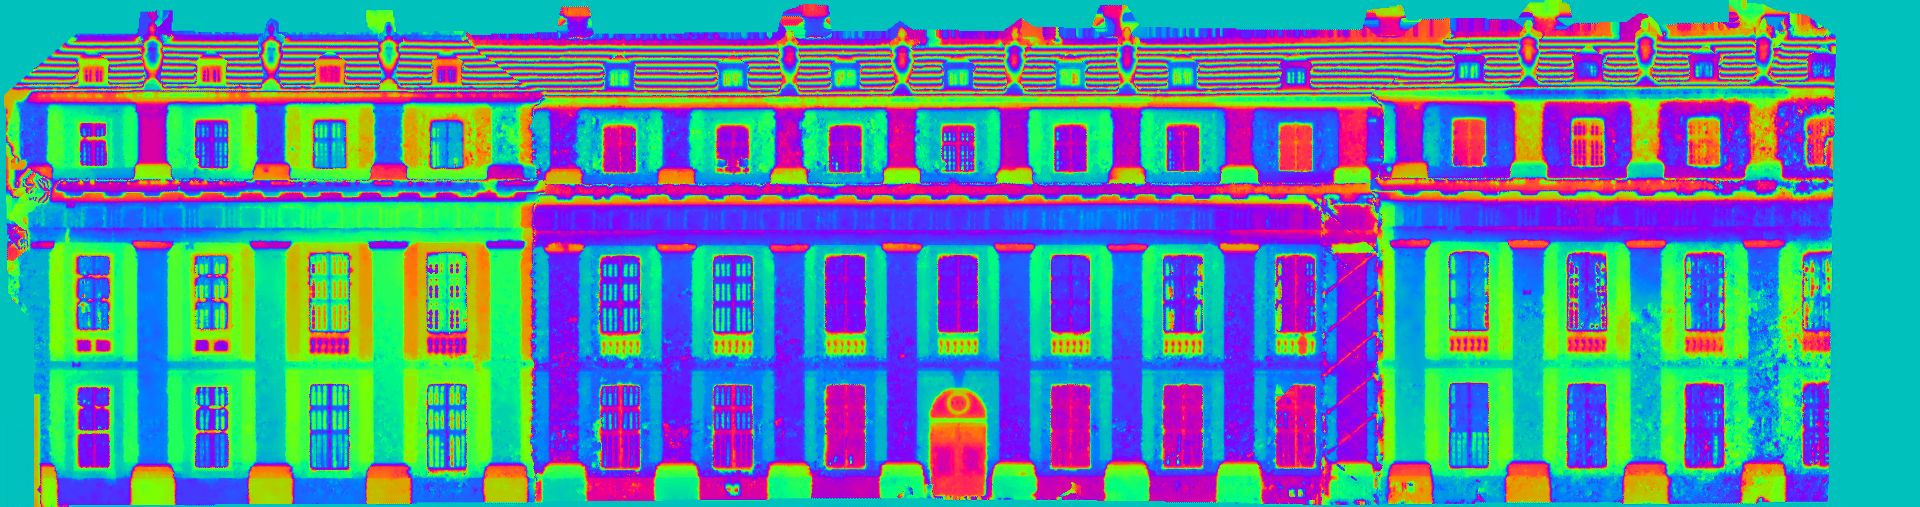
\includegraphics[width=160mm]{FIGS/Vincennes/MNE-OC.jpg}

\vspace{0.3cm}
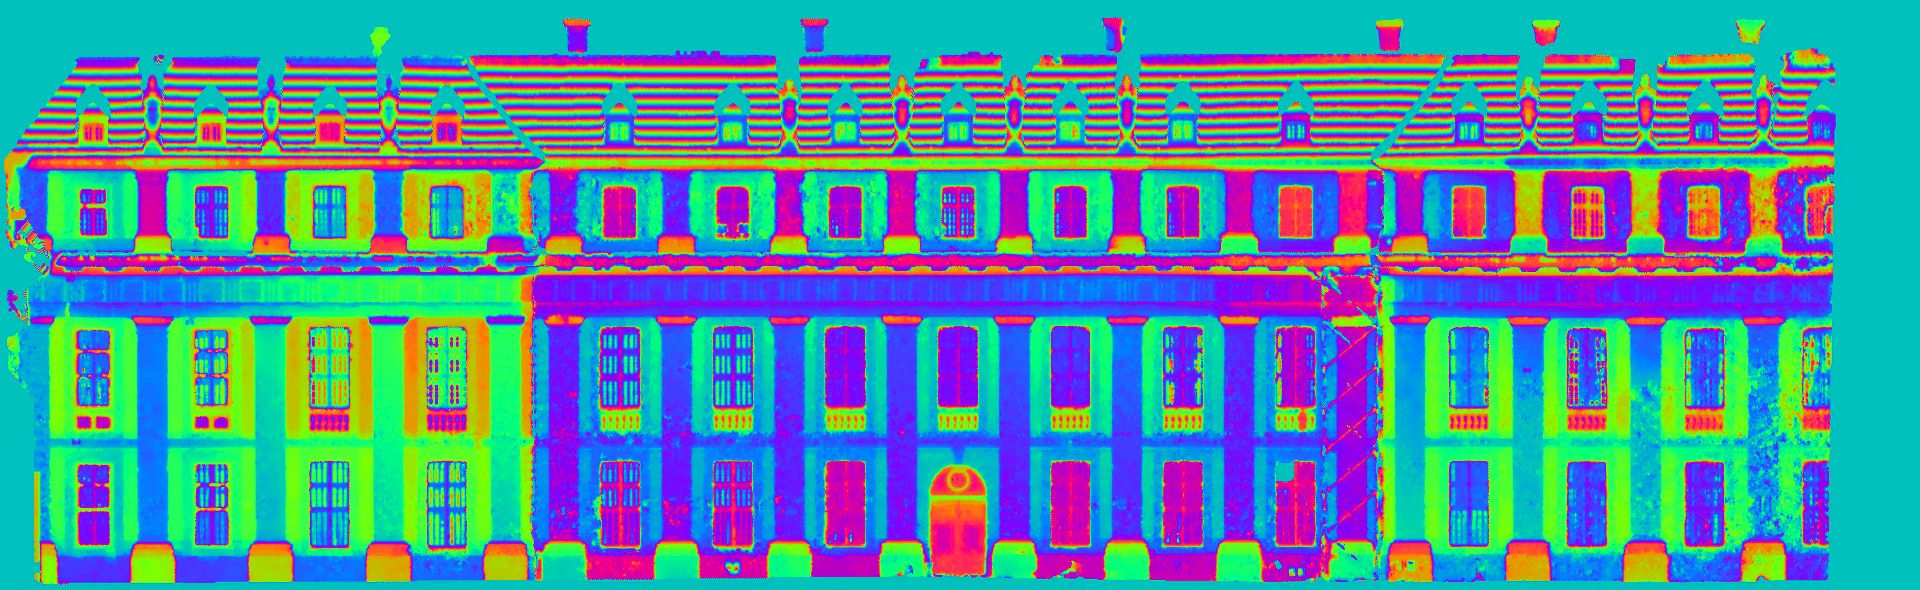
\includegraphics[width=160mm]{FIGS/Vincennes/MEN-Eucl.jpg}

\vspace{0.3cm}
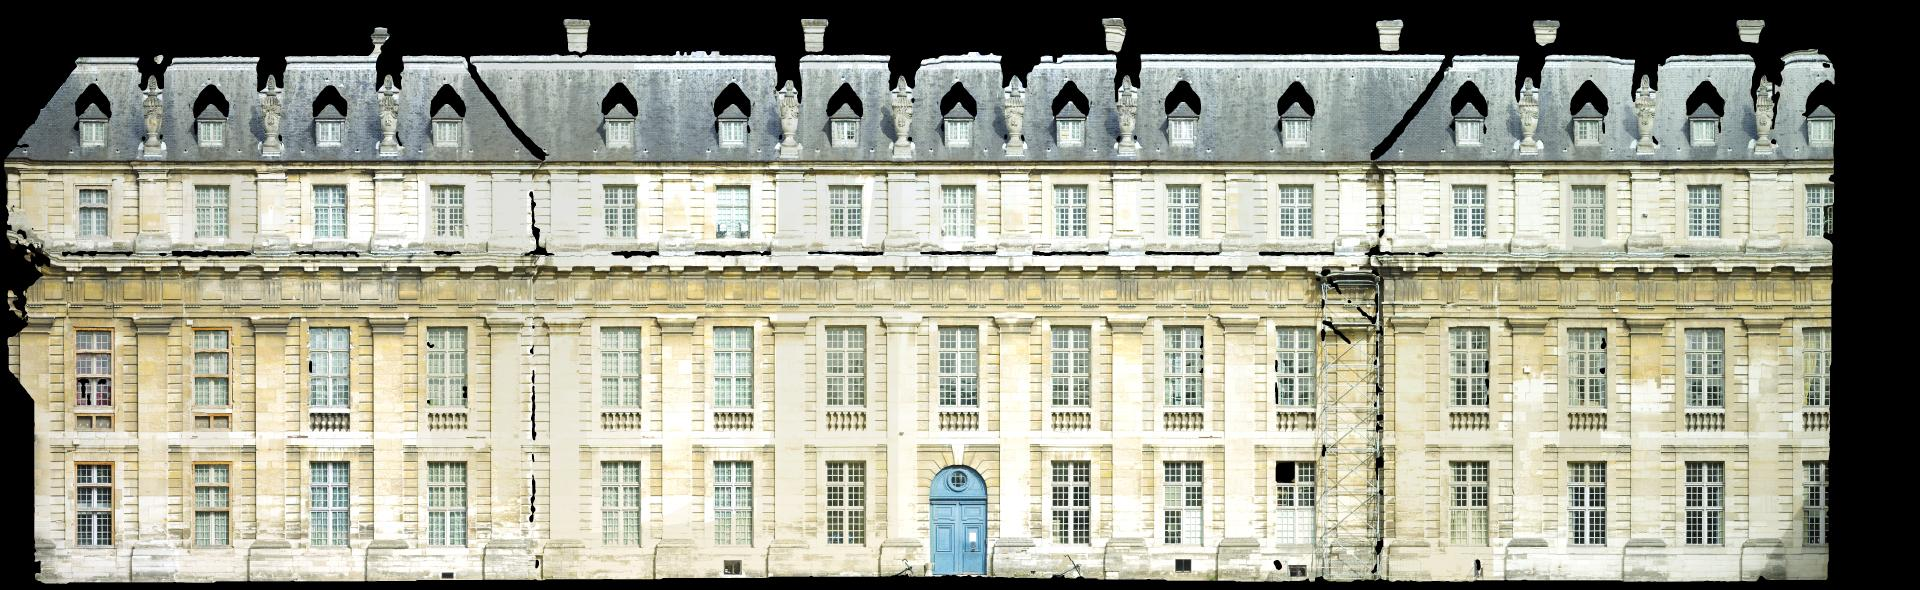
\includegraphics[width=160mm]{FIGS/Vincennes/Ortho-Eg-Test-Redr.jpg}

\end{center}
\caption{1-Depth map in ortho cylindric geometry, 2-The same, anamorphosed in euclidean
geometry, 3-Ortho photo in euclidean geometry}
\label{FIG:OK:Vincenne}
\end{figure}


Although all the tool described in this section are rather optimized 
for ortho-photo generation, it is still possible to generate 3D cloud points.
As usual in ground geometry, we use the result of matching for the 3D and
the ortho-photo for textures.
For example:


\begin{verbatim}
Nuage2Ply Malt-OC-F1/NuageImProf_Malt-Ortho-UnAnam_Etape_1.xml \
      Attr=Ortho-UnAnam-Malt-OC-F1/Ortho-Eg-Test-Redr.tif Scale=3

Nuage2Ply Malt-OC-F2/NuageImProf_Malt-Ortho-UnAnam_Etape_1.xml \
      Attr=Ortho-UnAnam-Malt-OC-F2/Ortho-Eg-Test-Redr.tif Scale=3
\end{verbatim}

The meta data file {\tt NuageImProf\_Malt-Ortho-UnAnam\_Etape\_1.xml} contains
all the information relative to the local repair use for computation  (inside
the {\tt <RepereGlob>} balise):

\begin{verbatim}
<?xml version="1.0" ?>
<XML_ParamNuage3DMaille>
     <NbPixel>5972 1834</NbPixel>
     <PN3M_Nuage>
..
     </PN3M_Nuage>
     <RepereGlob>
          <Ori>-0.00573682224569793675 -2.71135741550217935 -0.452115668474152133</Ori>
          <Ox>0.000296255688442622397 0.999999887087029138 -0.000371562236912849938</Ox>
          <Oy>-0.000437158066873386052 0.000371691728275074906 0.999999835369028367</Oy>
          <Oz>0.999999860562685972 -0.000296093208240548543 0.000437268133301418503</Oz>
     </RepereGlob>
...
  <Orientation>
....
  </Orientation>
...
</XML_ParamNuage3DMaille>
\end{verbatim}

The point cloud are then generated in the same global repair and are
naturally mergeable as can be seen on figure~\ref{FIG:TroidD:Vincenne}.


\begin{figure}
\begin{center}
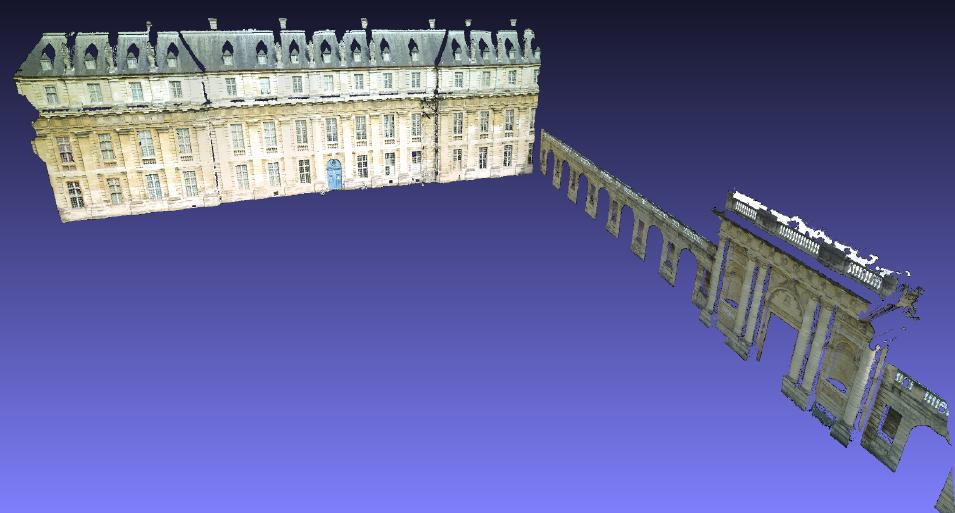
\includegraphics[width=160mm]{FIGS/Vincennes/Vinc3D.jpg}
\end{center}
\caption{Snapshot of two point clouds of the facade}
\label{FIG:TroidD:Vincenne}
\end{figure}

%-------------------------------------------------------------------
%-------------------------------------------------------------------
%-------------------------------------------------------------------

\section{The Saint-Michel de Cuxa data set}

%-------------------------------------------------------------------

\subsection{Description of the data set}
\label{Cuxa:DataSet}

On {\tt micmac\_data/ExempleDoc/} the directory {\tt MiniCuxha} contains
$48$ images of the St-Michel de Cuxa's abbey \footnote{they are low resolution images
to limit the  downloading time}. This data set illustrates how to
do a bundle adjustment with ground control points.

\begin{figure}
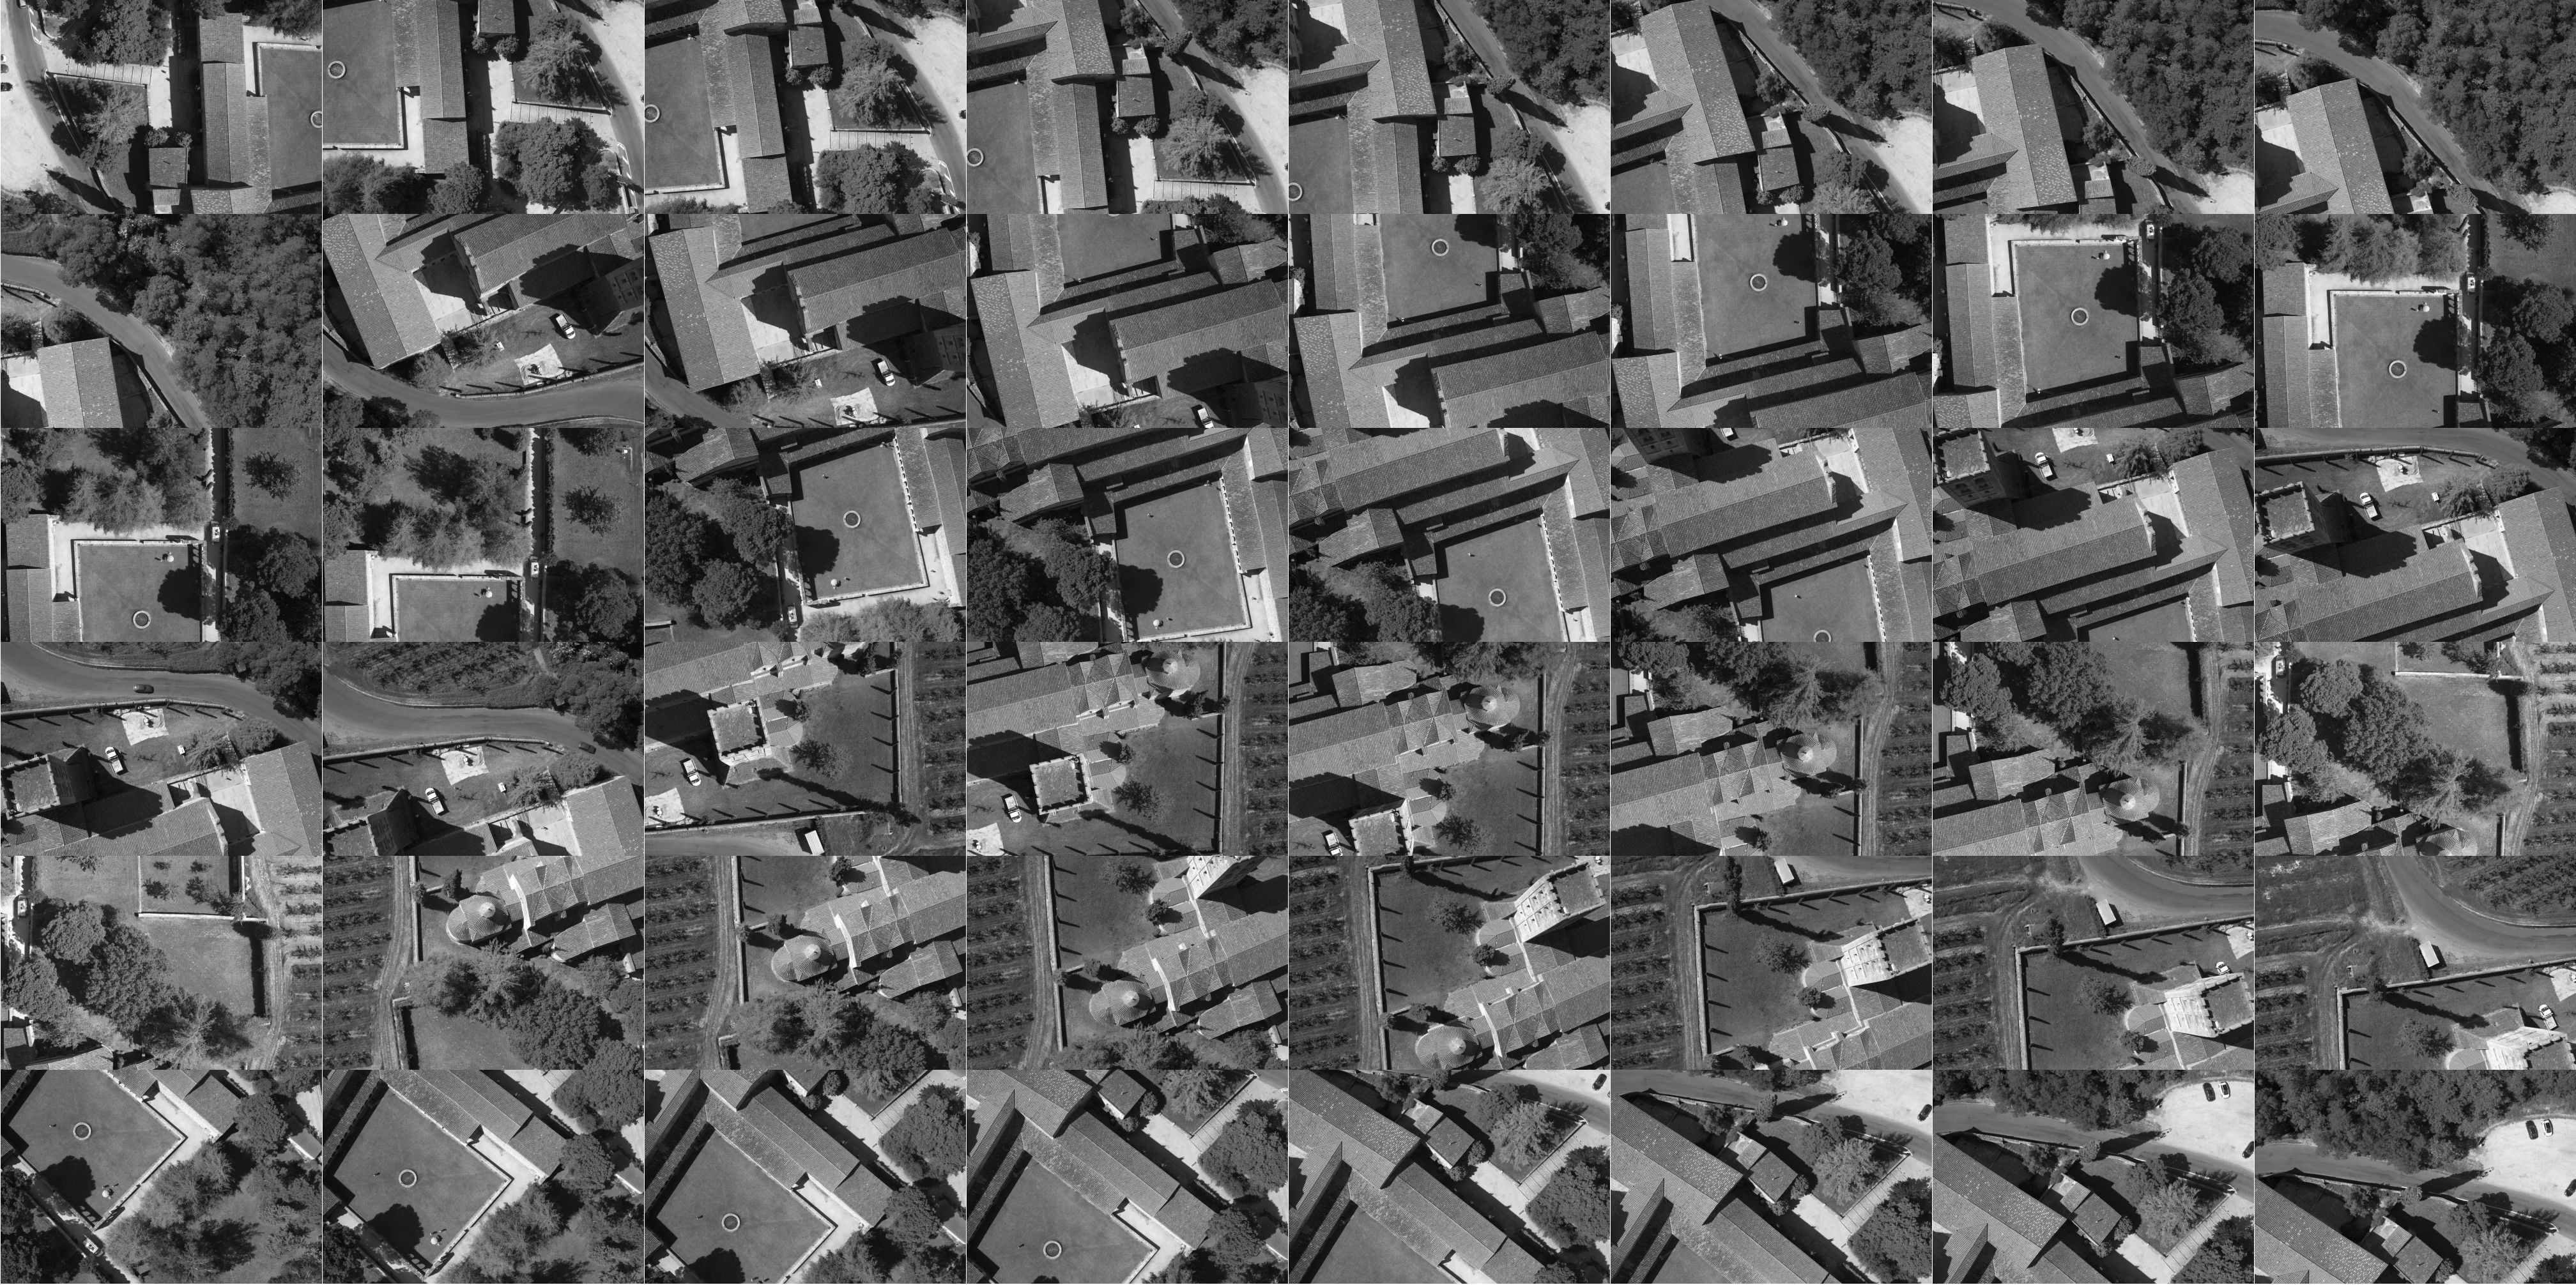
\includegraphics[width=120mm]{FIGS/SaintMicheldeCuxa/Planche.jpg}
\caption{Image of Saint-Michel de Cuxa's data set }
\label{FIG:Glob:Cuxa}
\end{figure}

\begin{figure}[H]
\begin{center}
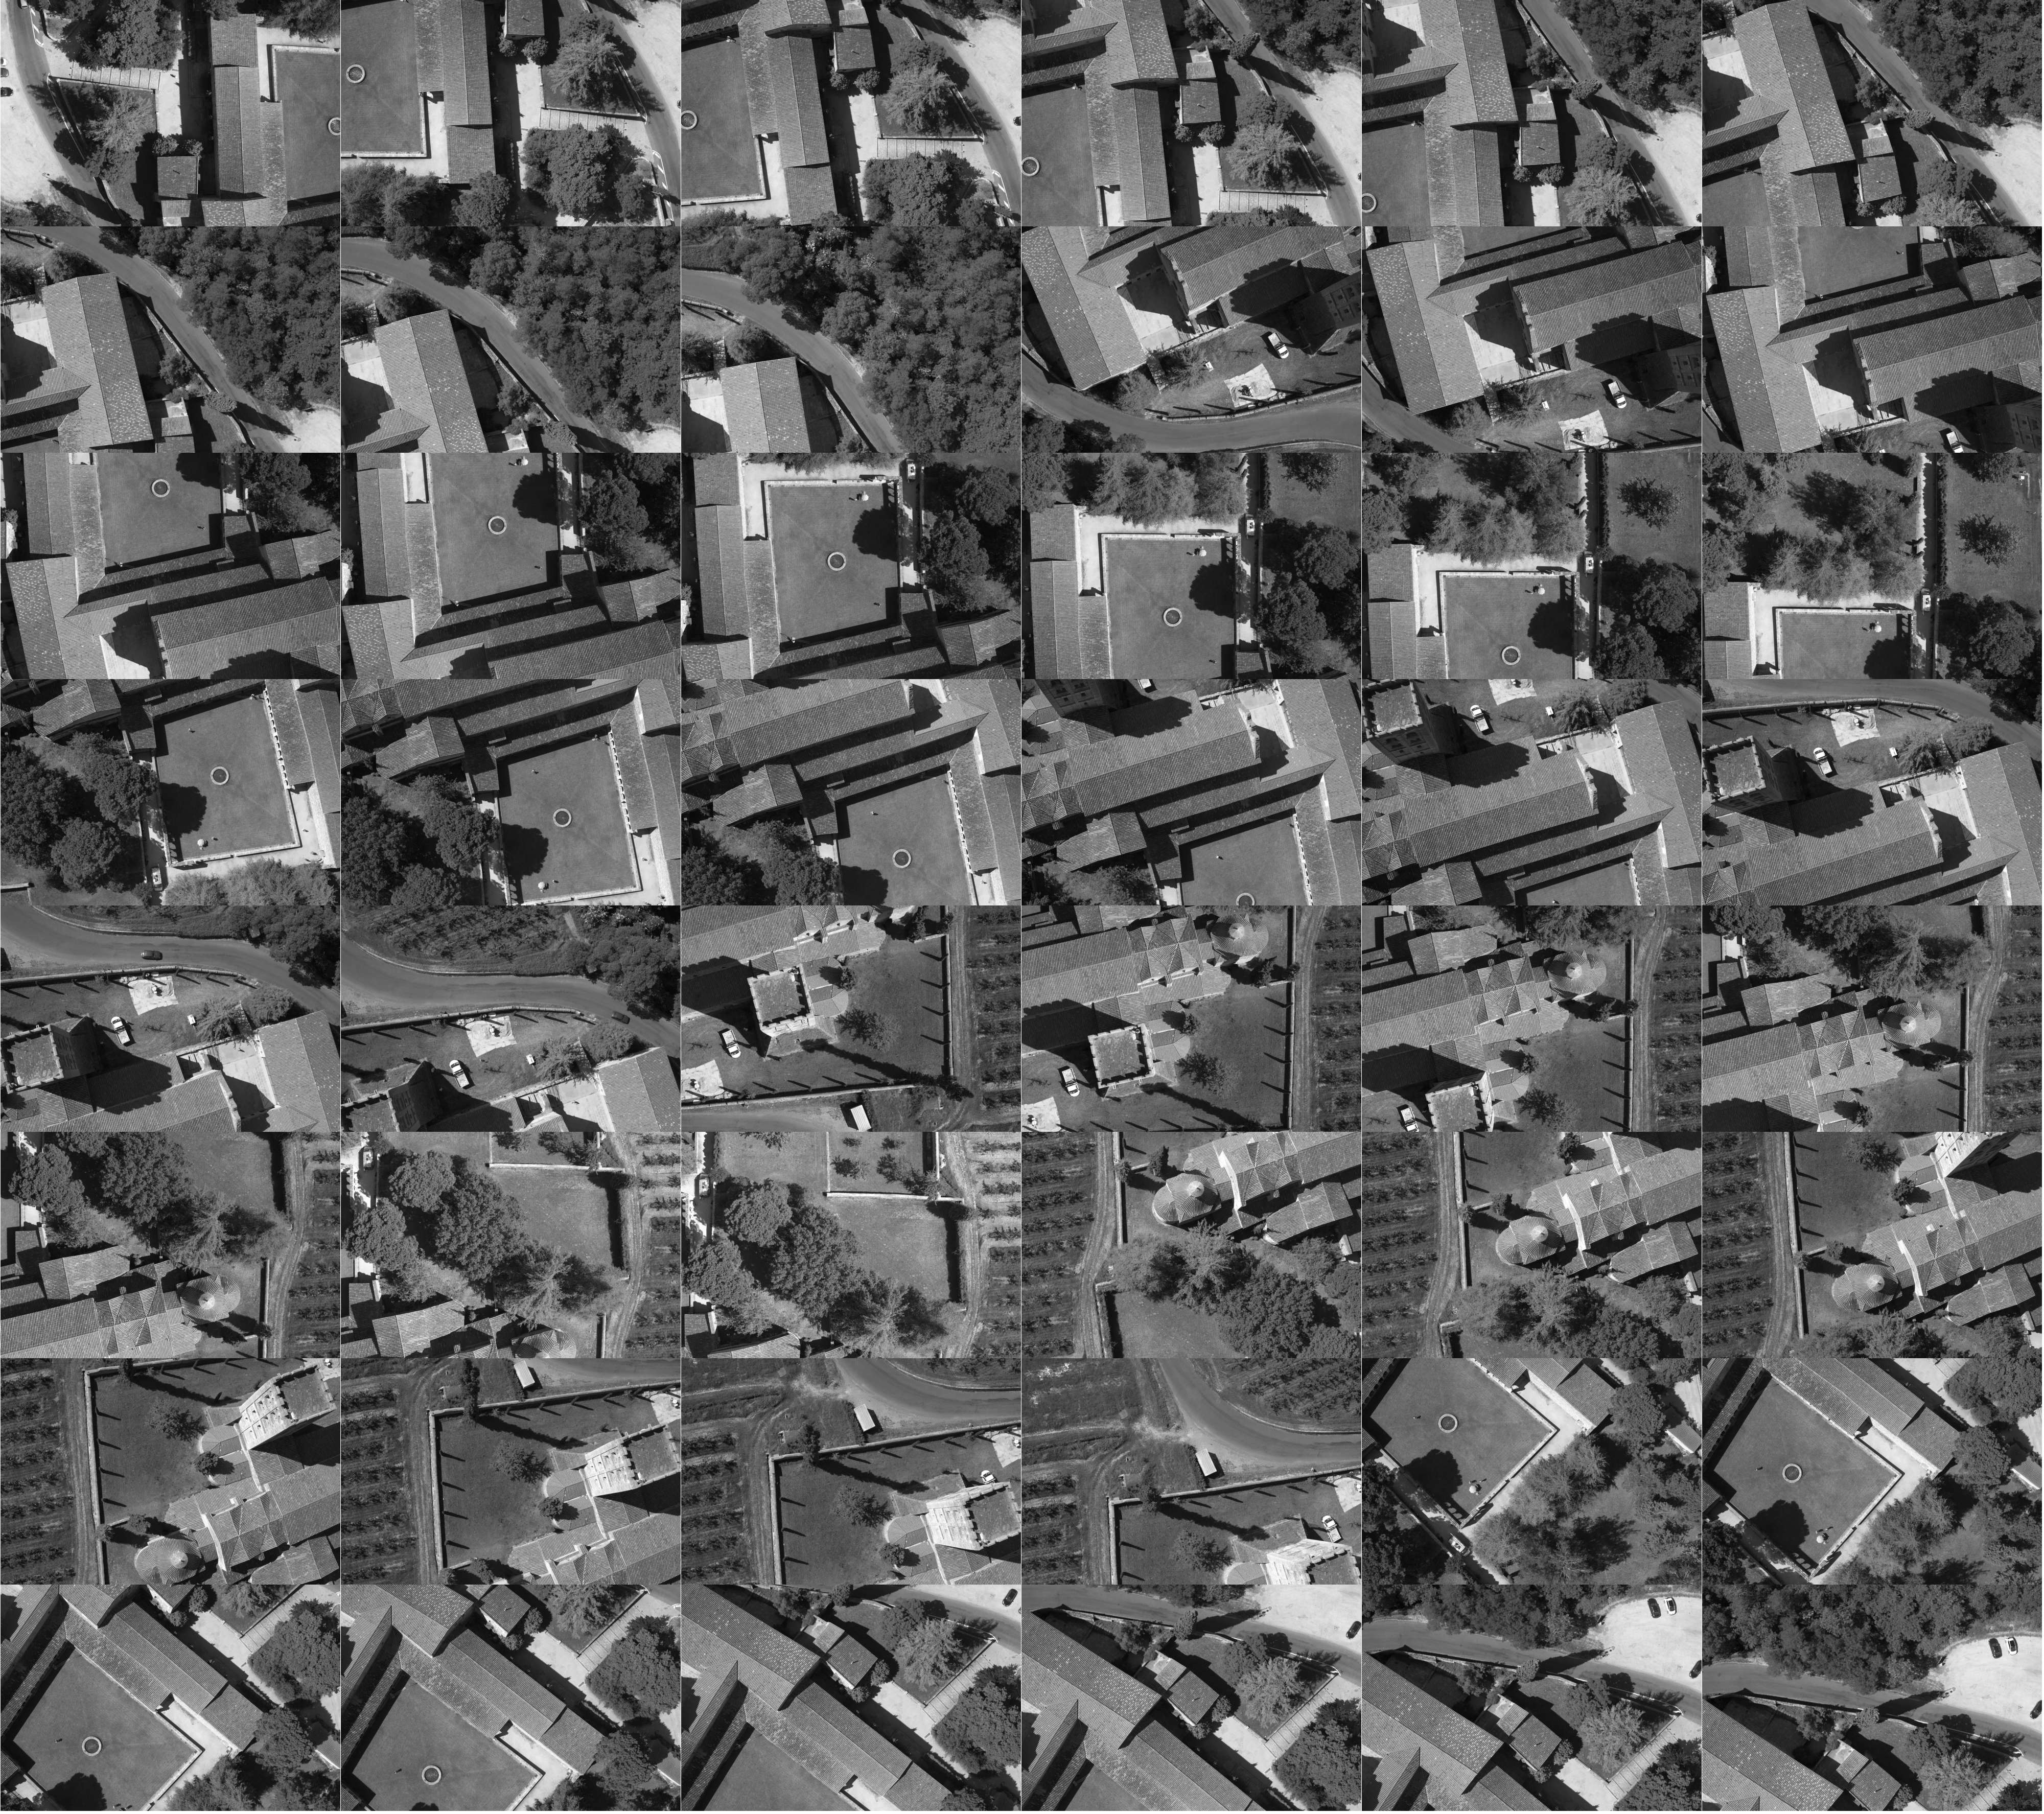
\includegraphics[width=160mm]{FIGS/Cuxa/Planche.jpg}
\caption{Image of Saint-Michel de Cuxa's data set }
\end{center}
\label{FIG:Glob:Cuxa}
\end{figure}

These images have been taken with an helicopter drone at an approximate height of ??? meters, in a typical aerial photogrammetric setup.

\vspace{\baselineskip}
The "standard pipeline" to do a bundle adjustment with ground control points with {\tt MicMac} is:
\begin{itemize}
\item compute images relative orientations, with {\tt Tapioca} and {\tt Tapas};
\item transform GCP coordinates into a local euclidean coordinate system, with {\tt GCPConvert};
\item measure image coordinates for a small set of GCP, with {\tt SaisieAppuisInit};
\item transform image relative orientations into the same local coordinate system, with {\tt GCPBascule};
\item measure image coordinates for all GCP, with {\tt SaisieAppuisPredic};
\item transform image relative orientations into the local coordinate system, with {\tt GCPBascule};
\item run the bundle adjustment, with {\tt Campari};
\item transform back relative orientations into an appropriate coordinate system, with {\tt ChgSysCo};
\item compute a rectified image, with {\tt Tarama};
\item make the matching with {\tt Malt};
\item generate the ortho image with {\tt Tawny};
\end{itemize}

\vspace{\baselineskip}
The file {\tt CmdAbbey.txt} contains all the commands needed to process these data.


%-------------------------------------------------------------------

\subsection{Computing tie points and relative orientations}

    %  -  -  -  -  -  -  -  -  -  -  -  -

\subsubsection{Tie points}

As usual, we want to compute matches between all pairs of calibration data set. This is done by:

\begin{verbatim}
Tapioca MulScale "Abbey-IMG_.*.jpg" 200 800
\end{verbatim}

    %  -  -  -  -  -  -  -  -  -  -  -  -  
	
\subsubsection{Relative orientation}

Then we want to make a first calibration with a subset of the whole data, and
use this calibration as an initial value to the global relative orientation of all images. This is done by:

\begin{verbatim}
Tapas RadialBasic "Abbey-IMG_(0248|0247|0249|0238|0239|0240).jpg" Out=Calib
Tapas RadialBasic "Abbey-.*.jpg" InCal=Calib Out=All-Rel
\end{verbatim}

We can verify that relative orientation was successful by checking the ``Residu Liaison Moyens'' (root mean square error) value that should be around 0.5 pixel.
We can also check visually the result of orientation running {\tt AperiCloud}, described in \ref{APERICLOUD}: 

\begin{verbatim}
AperiCloud  "Abbey-IMG_[0-9]*.jpg" All-Rel RGB=0
\end{verbatim}

This will generate the AperiCloud.ply file containing tie points and cameras locations. We can see that cameras are on the same plane, and that the relative orientations match the flight
plan:

\begin{figure}[H]
\begin{center}
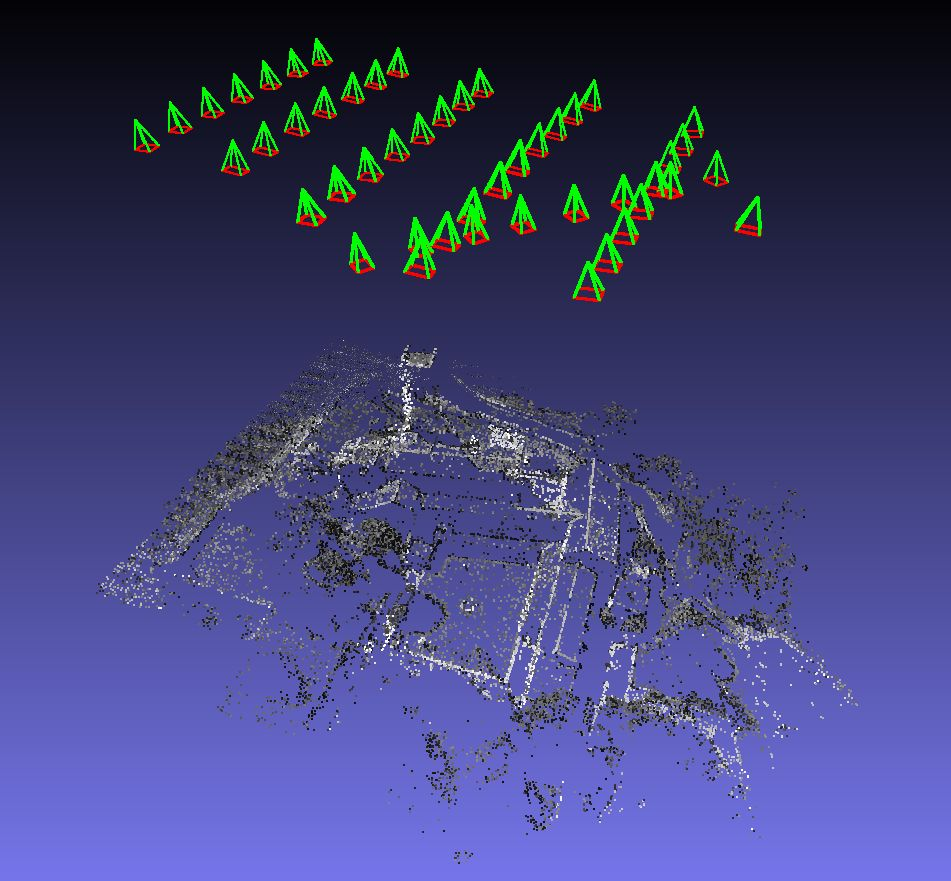
\includegraphics[width=180pt]{FIGS/Cuxa/AperiCloud.jpg}
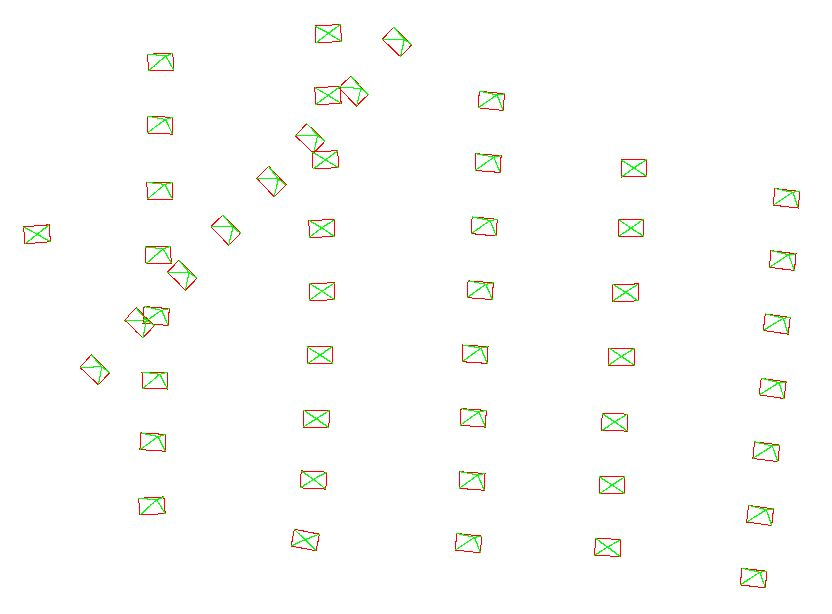
\includegraphics[width=208pt]{FIGS/Cuxa/Aero.jpg}
\caption{Result of relative orientation, computed with {\tt AperiCloud}, perspective and top view.}
\end{center}
\end{figure}

%-------------------------------------------------------------------

\subsection{GCP transforms}
		
    %  -  -  -  -  -  -  -  -  -  -  -  -

\subsubsection{Ground control point coordinates conversion}

In this use case, we have got ground control points expressed in {\tt WGS84} system. We need to convert them into a local euclidean coordinate system. The important thing is that the local system is euclidean, because all the {\tt MicMac} tools
need this assumption to solve equations. Most of the cartographic coordinate systems are not euclidean systems, so we define a local tangent system, defined around a 3D point and its tangent plane, that will lead to a geometry compliant with {\tt MicMac}'s one.
This is done with the {\tt GCPConvert} tool (detailed in \ref{GCPConvert}):

\begin{verbatim}
GCPConvert "#F=N_X_Y_Z_I" F120601.txt ChSys=DegreeWGS84@SysCoRTL.xml Out=AppRTL.xml
\end{verbatim}

\subsubsection{Ground control point image coordinates input}

To add image coordinates measures, we can use the {\tt SaisieAppuisInit} interface in Linux (detailed in \ref{SaisieAppuisInit}):

\begin{verbatim}
SaisieAppuisInit  "Abbey-IMG_0211.jpg"  All-Rel  NamePointInit.txt  MesureInit.xml
\end{verbatim}

This will create two {\tt Xml} files {\tt MesureInit-S2D.xml} and {\tt MesureInit-S3D.xml}, which respectively contain images coordinates and corresponding 3D coordinates, computed by spatial resection.

\subsubsection{Bascule}

Now we can transform images relative orientations, as computed with Tapas, expressed in an arbitrary coordinate system,
into the local euclidean coordinate system, using 2D images coordinates measures and 3D corresponding ground control points. 

\begin{verbatim}
GCPBascule "Abbey-.*jpg" All-Rel  RTL-Init  AppRTL.xml  MesureInit-S2D.xml 
\end{verbatim}

Once the images relative orientations have been transformed back in local euclidean coordinate system, one can verify that Z coordinates for the whole data set is nearly constant, which corresponds to the data acquisition setup.

\vspace{\baselineskip}
Possible error: "{\tt Not enough samples (Min 3) in cRansacBasculementRigide}". It means that there is not enough points to compute a Bascule transform. You should add more points with {\tt SaisieAppuisInit}:
at least 3 GCP whose projection are known in at least 2 images are needed.

\subsubsection{Adding points with predictive interface {\tt SaisieAppuisPredic}}

When the global transform between ground control points and image relative orientations is known, we can switch to the predictive interface {\tt SaisieAppuisPredic} which will display the remaining ground control points, loaded from the {\tt Xml} file {\tt AppRTL.xml}.
You need to adjust points image location and validate them.

\begin{verbatim}
SaisieAppuisPredic  "Abbey-.*jpg" RTL-Init AppRTL.xml  MesureFinale.xml
\end{verbatim}

\subsubsection{Bascule}

Again we can transform images relative orientations, this time with a more substantial number of images measures, which will give a better transform.
\begin{verbatim}
GCPBascule "Abbey.*jpg" All-Rel  RTL-Bascule AppRTL.xml MesureFinale-S2D.xml
\end{verbatim}

%-------------------------------------------------------------------

\subsection{Bundle adjustment with ground control points}

Now we can run a constrained bundle adjustment combining ground control points and tie points, with the {\tt Campari} command, described in \ref{CAMPARI}.

\begin{verbatim}
Campari "Abbey.*.jpg"  RTL-Bascule RTL-Compense GCP=[AppRTL.xml,0.1,MesureFinale-S2D.xml,0.5]
\end{verbatim}

%-------------------------------------------------------------------

\subsection{Post-processing}

\subsubsection{Coordinate system backward transform}

Then one can transform coordinates from the local euclidean coordinate system to a geographic coordinate system, and compute ortho-images which can be superimposed on vectorial maps (and \textit{vice versa}). 
For example, if we want to transform our data into the sinusoidal projection, for which we have got a file {\tt SysCoSinus90W.xml} storing the transformation parameters, the command is:

\begin{verbatim}
ChgSysCo  "Abbey.*.jpg" RTL-Compense SysCoRTL.xml@SysCoSinus90W.xml Sin90

Tarama  "Abbey.*.jpg" Sin90

Malt Ortho  "Abbey.*.jpg" Sin90 SzW=1 AffineLast=false DefCor=0.0

Tawny Ortho-MEC-Malt/
\end{verbatim}

\begin{figure}[H]
\begin{center}
\includegraphics[width=150mm]{FIGS/Cuxa/Sinus-Ortho-Eg-Test-Redr.jpg}
\caption{Image rectification in sinusoidal projection, with {\tt Tarama}}
\end{center}
\end{figure}

%\begin{figure}[H]
%\begin{center}
%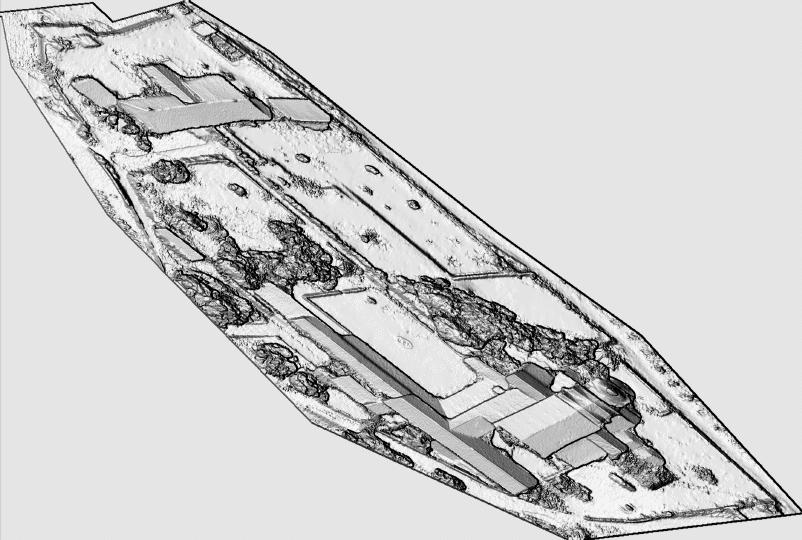
\includegraphics[width=150mm]{FIGS/Cuxa/SinusShade.jpg}
%\caption{Shading in sinusoidal projection, with {\tt GrShade}}
%\end{center}
%\end{figure}

The result is ugly, but if we have a look to the global earth mapping with sinusoidal projection, it is obvious that we cannot have a good representation at the european longitude with the sinusoidal projection.

\begin{figure}[H]
\begin{center}
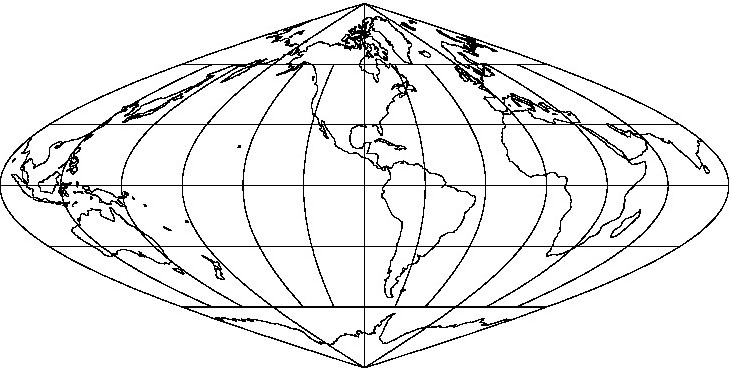
\includegraphics[width=182pt]{FIGS/Cuxa/Sinus90.jpg}
\caption{Sinusoidal projection, with Central Meridian $90\,^{\circ}$W}
\end{center}
\end{figure}

What we expect would be more like the result of a projection in Lambert93 coordinate system:

\begin{verbatim}
ChgSysCo  "Abbey.*.jpg" RTL-Compense SysCoRTL.xml@Lambert93 L93

Tarama  "Abbey.*.jpg" L93

Malt Ortho  "Abbey.*.jpg" L93 SzW=1 AffineLast=false DefCor=0.0

Tawny Ortho-MEC-Malt/
\end{verbatim}

\begin{figure}[H]
\begin{center}
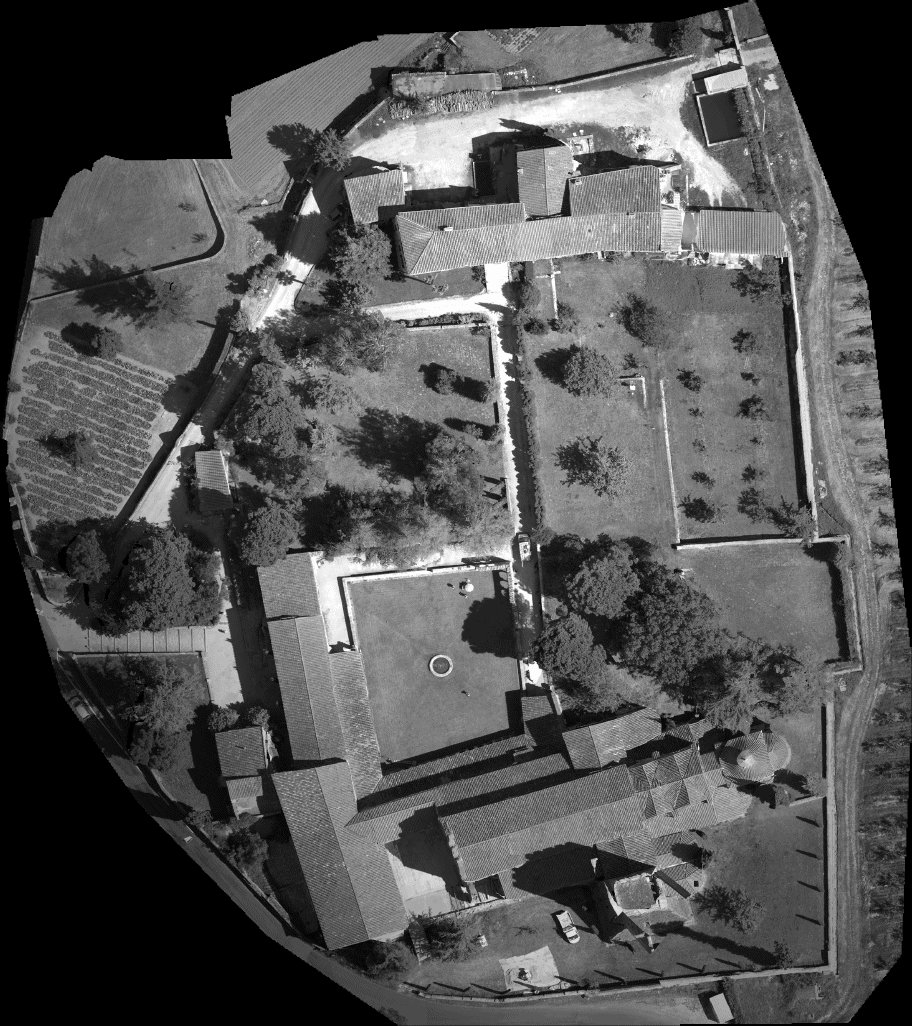
\includegraphics[width=160mm]{FIGS/Cuxa/L93-Ortho-Eg-Test-Redr.jpg}
\caption{Image rectification in Lambert93 projection, with {\tt Tawny}}
\end{center}
\end{figure}

\begin{figure}
\begin{center}
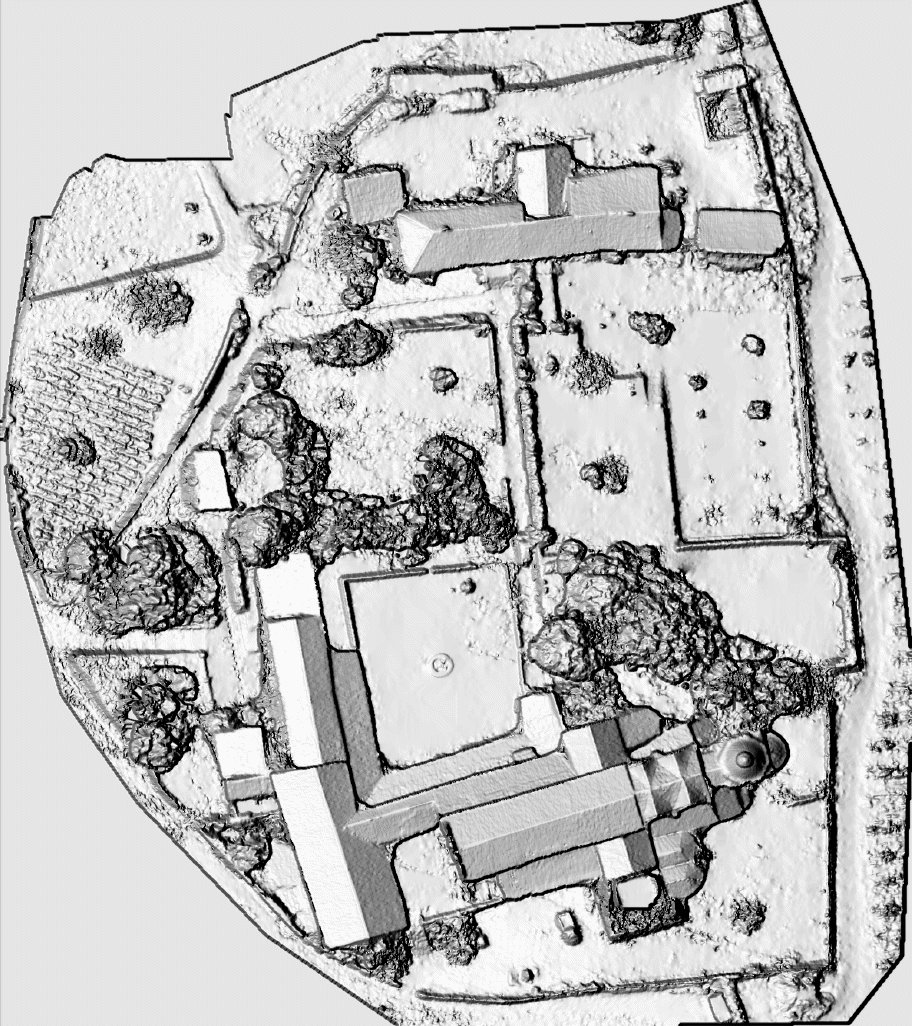
\includegraphics[width=160mm]{FIGS/Cuxa/L93-Shade.jpg}
\caption{Shading in Lambert93 projection, with {\tt GrShade}}
\end{center}
\end{figure}


